%% ****** Start of file apstemplate.tex ****** %
%%
%%
%%   This file is part of the APS files in the REVTeX 4.2 distribution.
%%   Version 4.2a of REVTeX, January, 2015
%%
%%
%%   Copyright (c) 2015 The American Physical Society.
%%
%%   See the REVTeX 4 README file for restrictions and more information.
%%
%
% This is a template for producing manuscripts for use with REVTEX 4.2
% Copy this file to another name and then work on that file.
% That way, you always have this original template file to use.
%
% Group addresses by affiliation; use superscriptaddress for long
% author lists, or if there are many overlapping affiliations.
% For Phys. Rev. appearance, change preprint to twocolumn.
% Choose pra, prb, prc, prd, pre, prl, prstab, prstper, or rmp for journal
%  Add 'draft' option to mark overfull boxes with black boxes
%  Add 'showkeys' option to make keywords appear
\documentclass[aps,prl,preprint,groupedaddress]{revtex4-2}
%\documentclass[aps,prl,preprint,superscriptaddress]{revtex4-2}
%\documentclass[aps,prl,reprint,groupedaddress]{revtex4-2}

% You should use BibTeX and apsrev.bst for references
% Choosing a journal automatically selects the correct APS
% BibTeX style file (bst file), so only uncomment the line
% below if necessary.
%\bibliographystyle{apsrev4-2}

\usepackage{graphicx}
%\usepackage{epstopdf,epsfig}
\usepackage{newtxtext}
\usepackage{newtxmath}
\usepackage{natbib}
\usepackage{hyperref}
\usepackage{mathtools}
\usepackage{commath}

\newtheorem{lemma}{Lemma}
\newtheorem{theorem}{Theorem}
\newtheorem{corollary}{Corollary}
\newcommand{\RomanNumeralCaps}[1]
\linenumbers


% Bryan's Marcros
\renewcommand{\aa}{\mathbf{a}}
\newcommand{\bd}{\partial}
\newcommand{\dd}{\mathbf{d}}
\newcommand{\DD}{\mathcal{D}}
\newcommand{\SSS}{\mathcal{S}}
\newcommand{\eeta}{\boldsymbol{\eta}}
\newcommand{\FF}{\mathbf{F}}
\newcommand{\GG}{\mathbf{G}}
\newcommand{\JJ}{\mathbf{J}}
\newcommand{\nnu}{\boldsymbol{\nu}}
\newcommand{\ttau}{\boldsymbol{\tau}}
\newcommand{\ssigma}{\boldsymbol{\sigma}}
\newcommand{\rr}{\mathbf{r}}
\newcommand{\RR}{\mathbf{R}}
\renewcommand{\SS}{\mathbf{S}}
\newcommand{\xx}{\mathbf{x}}
\newcommand{\zz}{\mathbf{z}}
\newcommand{\XX}{\mathbf{X}}
\newcommand{\uu}{\mathbf{u}}
\renewcommand{\vv}{\mathbf{v}}
\newcommand{\yy}{\mathbf{y}}
\newcommand{\pderiv}[2]{\frac{\partial #1}{\partial #2}}
\newcommand{\jump}[1]{[\![ #1 ]\!]}


\begin{document}

% Use the \preprint command to place your local institutional report
% number in the upper righthand corner of the title page in preprint mode.
% Multiple \preprint commands are allowed.
% Use the 'preprintnumbers' class option to override journal defaults
% to display numbers if necessary
%\preprint{}

%Title of paper
\title{Collective behavior of Suspended Janus Particles via an Integral Equation Method}

% repeat the \author .. \affiliation  etc. as needed
% \email, \thanks, \homepage, \altaffiliation all apply to the current
% author. Explanatory text should go in the []'s, actual e-mail
% address or url should go in the {}'s for \email and \homepage.
% Please use the appropriate macro foreach each type of information

% \affiliation command applies to all authors since the last
% \affiliation command. The \affiliation command should follow the
% other information
% \affiliation can be followed by \email, \homepage, \thanks as well.
\author{Szu-Pei Fu}
\email{sfu17@fordham.edu}
%\homepage[]{Your web page}
%\thanks{}
%\altaffiliation{}
\author{Rolf Ryham}
\email{rryham@fordham.edu}
\affiliation{Department of Mathematics, Fordham University, Bronx, New York 10458, USA}

\author{Bryan Quaife}
\email{bquaife@fsu.edu}
 \affiliation{Department of Scientific Computing, Florida State University, Tallahassee, Florida 32306, USA}
 \author{Y.-N. Young}
 \email{yyoung@njit.edu}
 \affiliation{Department of Mathematical Sciences, New Jersey Institute of Technology, Newark, New Jersey 07102, USA
 }




%Collaboration name if desired (requires use of superscriptaddress
%option in \documentclass). \noaffiliation is required (may also be
%used with the \author command).
%\collaboration can be followed by \email, \homepage, \thanks as well.
%\collaboration{}
%\noaffiliation

\date{\today}

\begin{abstract}
% insert abstract here
\end{abstract}

% insert suggested keywords - APS authors don't need to do this
%\keywords{}

%\maketitle must follow title, authors, abstract, and keywords
\maketitle

% body of paper here - Use proper section commands
% References should be done using the \cite, \ref, and \label commands
\section{Introduction}
% Put \label in argument of \section for cross-referencing
%\section{\label{}}


\subsection{}


\subsubsection{}






%%%


\section{Governing Equations}


\subsection{Screened Laplace Mobility Problem}


The mathematical formulation is a nonlinear system for the dynamics of a
collection of particles. The interactions come from a system of 
partial differential equations (PDEs) that comprise hydrodynamic
interactions and hydrophobic interactions.
The hydrodynamic interactions come from the mobility problem for rigid
particles immersed in a viscous solvent. We then use a
second-order Adams-Bashforth method to update the particle configuration.
Assuming inertial terms are
negligible, the particle motion is goverened by the Stokes equations
\begin{alignat}{3}
\label{eq:stokes}
  -\mu \Delta \uu + \nabla p &= \mathbf{0},     && \xx \in \Omega, \\
  \nabla\cdot \uu &= 0, \qquad && \xx \in \Omega, \\
  \uu - \uu_\infty &\to \mathbf{0}, && |\xx| \to \infty,
\end{alignat}
where $\uu$ is the velocity and $p$ is the pressure of the solvent,
$\uu_\infty$ is the background flow, and $\mu$ is the constant solvent
viscosity. The domain $\Omega = \Omega(t)$ is the fluid region surrounding the
particles and changes shape as the particles move.
Since the particles are rigid, the solvent velocity satisfies
a no-slip boundary condition for a rigid body motion 
on the particle boundary $\Gamma_i$ with translational velocity $\vv_i$
and angular velocity $\omega_i$.
Given imposed forces acting on each
particle, the mobility problem consists of finding
translational and angular velocities so that viscous fluid forces
balance the imposed forces.

The hydrophobic interactions come from the tendency of particles to
minimize the free energy of the structure of the surrounding water
molecules. The free energy functional takes the form 
\begin{equation}
\label{eq:free_energy}
  F[u] = C \int_{\Omega} \left(\rho |\nabla u|^2 + \rho^{-1} f(u)\right)
  \,d\xx,
\end{equation}
where $u$ is an order parameter for the structure of water, $\rho$ is a
decay length, $C$ is a constant, and $f(u)$ is a potential.
Hydrogen-bond persistence times are on the order of picoseconds
which is much smaller than characteristic time for 
particle motion. % \cite{MaGa13}.
Thus we assume $u$ minimizes $F[u]$ for all times.
Assuming appropriate conditions on $f(u)$,% (\cite{evans10}, \S 8.2),
 $u$ is bounded and satisfies the Euler-Lagrange equation
\begin{equation}
\label{eq:SL}
-\rho^2 \Delta u + \tfrac{1}{2}f'(u) = 0  \text{ in } \Omega,\quad u = g,
\text{ on } \bd\Omega.
\end{equation}
The boundary condition $g$ is a material label that is transported with
the particle (Figure~\ref{fig:bcs}).

The particles lower the free energy $F[u]$ of the surrounding water
by moving. We calculate the rate of change of $F[u]$ using
variation of the domain. % ~\cite{Fu2018_SIAM,Bandle2015, Schiffer1954, Grinfeld2010}.
Carrying out this variation yields a stress  
\begin{align}
  \label{eq:stress}
\mathbf{T}
= C \left[ \rho^{-1} f(u) \mathbf{I}
  + \rho \left(|\nabla u|^2 \mathbf{I} - 2\nabla u \nabla u^T\right)\right].
\end{align}
The imposed forces and torques come from the integration of $\mathbf{T}$
along the particle boundary.
These forces and torques couple the Stokes equations \eqref{eq:stokes},
to semilinear elliptic equation \eqref{eq:SL}.
Solving for the translational and rotational velocities gives the
particle evolution.

\begin{align}
  \label{eq:velocity}
  \uu(\xx) = \uu_\infty(\xx) + \DD[\eeta](\xx) + 
    \sum_{i=1}^{N_b} \left(\SS(\xx,\aa_i) \cdot \FF_i + 
    \RR(\xx,\aa_i) T_i\right), \quad \xx \in \Omega.
\end{align}
%
where the density function $\eeta$, translation velocity $\vv_i$ and angular velocity $\omega_i$ satisfy

\begin{alignat}{3}
  \nonumber
  \vv_i + \omega_i (\xx - \aa_i)^\perp &= \uu_\infty(\xx)
    -\frac{1}{2} \eeta(\xx) + \DD[\eeta](\xx) \\
  \label{eq:SKIE}
    + \sum_{j=1}^{N_b} &
    \left(\SS(\xx,\aa_j) \cdot \FF_j + \RR(\xx,\aa_j) T_j\right),
    \quad &&\xx \in \Gamma_i,\: i=1,\ldots,N_b, \\
  \label{eq:mobility1}
  \int_{\Gamma_i} \eeta \, \dif s &= \mathbf{F}_i, 
  &&i = 1,\ldots,N_b, \\
  \label{eq:mobility2}
  \int_{\Gamma_i} \eeta \cdot (\xx-\aa_i)^\perp \, \dif s &= T_i,
  &&i = 1,\ldots,N_b.
\end{alignat}


\subsection{Normal Derivative of Double Layer Potential and HAP Energy}

We adopt the double layer potential to express the solution of \eqref{eq:SL} where the condition is $f(u)=u^2$. Then it is given by 
\begin{align}
\label{eq:energy_BIE}
u({\bf x}) = \DD[\sigma](\xx) = \int_\Gamma \frac{\partial G(\xx-\yy)}{\partial \nnu_\yy}\sigma(\yy)\, \dif s_\yy,
\end{align}
%
where $G(\xx)$ is the fundamental solution to the screened Laplace equation \eqref{eq:SL} and $\nnu$ is the outward normal.
Since the free energy functional can be written as 
\begin{align}
\label{eq:free_energy2}
  E[u(\xx)] &= C\rho \int_\Gamma u \frac{\partial u}{\partial \nnu}  \,\dif s, \quad \xx\in\Gamma_i,
\end{align}
%
we can then refer to the identity (\cite{Hsiao2008}, \S 1.2) to calculate this boundary integral equation without evaluating the normal derivative of the double layer potential directly.

Consider
\begin{align}
\nnu_\xx \cdot \nabla_\zz u(\zz) &=\nnu_\xx \cdot \nabla_\zz \int_\Gamma \frac{\partial G(\zz-\yy)}{\partial \nnu_\yy}\sigma(\yy) \,\dif s_\yy\\
&=\int_\Gamma \nnu_\xx\cdot \left(\nabla_\zz\nabla_\yy^\top  G(\zz-\yy)\right)\cdot \nnu_\yy\sigma(\yy)  \,\dif s_\yy\\
&=-\int_\Gamma \nnu_\xx\cdot \left(\nabla_\yy\nabla_\yy^\top G(\zz-\yy)\right)\cdot\nnu_\yy\sigma(\yy)\ \dif s_\yy\\
&=-\int_\Gamma {\bf t}_\xx\cdot\Delta_\yy G(\zz-\yy) {\bf t}_\yy \sigma(\yy)\ \dif s_\yy+\int_\Gamma({\bf t}_\xx\cdot\nabla_\yy)({\bf t}_\yy\cdot\nabla_\yy G(\zz-\yy))\sigma(\yy)\ \dif s_\yy\\
&= -\int_\Gamma {\bf t}_\xx\cdot\frac1\rho^2 G(\zz-\yy) {\bf t}_\yy \sigma(\yy)\ \dif s_\yy - 
({\bf t}_\xx\cdot\nabla_\zz)\int_\Gamma \frac{\partial G(\zz-\yy)}{\partial s_\yy}\sigma(\yy)\ \dif s_\yy\\
&= -\frac1\rho^2 {\bf t}_\xx\cdot \int_\Gamma G(\zz-\yy){\bf t}_\yy \sigma(\yy)\ \dif s_\yy + 
({\bf t}_\xx \cdot \nabla_\zz)\int_\Gamma G(\zz-\yy)\frac{\partial \sigma(\yy)}{\partial s}\ \dif s_\yy.
\end{align}
%
Here ${\bf t}_\xx$ is the tangent vector at the point $\xx$ and $d/ds$ is the arclength derivative.
Letting $\zz\to\xx\in\Gamma$, we obtain
%
\begin{equation}
\label{eq:normal_deriv}
\frac{\partial}{\partial \nnu_\xx} \DD[\sigma](\xx) = -\frac1\rho^2 {\bf t}_\xx\cdot \SSS[\sigma{\bf t}](\xx) + \frac{\partial}{\partial s}\SSS\left[\frac{\partial \sigma}{\partial s}\right](\xx).
\end{equation}
%

Substituting \eqref{eq:normal_deriv} to \eqref{eq:energy_BIE} provides the total energy calculation
throughout this paper and this expression takes the advantage of not calculating the quadruple layer potential.

%Suppose we split the solution to the screened Laplace boundary value problem~\eqref{eq:SL}
%into smooth portion $w_i$ and singular portion $u_i$. That is, 
%\begin{equation}
%w_i({\bf x}) = u({\bf x}) - u_i = u({\bf x}) - \int_{\Gamma_i }\left(\pderiv{}{\nnu_\yy}
%    K_0 \left(\frac{|\xx - \yy|}{\rho}\right)\right) \sigma_i(\yy) \,
%    \dif s_\yy, \quad \xx \in \Gamma_i.
%\end{equation}
%Consider the case when $f(u)=u^2$ in~\eqref{eq:free_energy}, we can rewrite the free energy functional as 
%
%\begin{align}
%\label{eq:free_energy2}
%  E[u(\xx)] &= C\rho \sum_{i=1}^{N_b}\int_{\Gamma_i} u \frac{\partial u}{\partial \nnu}  \,\dif s
%= C\rho\sum_{i=1}^{N_b}\int_{\Gamma_i} u \left(\frac{\partial w_i}{\partial \nnu}+\frac{\partial u_i}{\partial \nnu} \right) \, \dif s, \quad \xx\in\Gamma_i.
%\end{align}
%%%%
%Follow the divergence theorem on the last term in the equation above and denote $g_i(x)$ as the boundary data on $\Gamma_i$, we obtain
%\begin{align}
%\label{eq:free_energy3}
%  E[u(\xx)] &= C\rho\sum_{i=1}^{N_b}\left(\int_{\Gamma_i} u \frac{\partial w_i}{\partial \nnu} \,\dif s  + \int_{\mathbb{R}^n\setminus \overline{U}_i} \left( \nabla u \cdot\nabla u_i + u\Delta u_i\right) \,\dif \xx\right)\\
%%
%&= C\rho\sum_{i=1}^{N_b}\left(\int_{\Gamma_i} u \frac{\partial w_i}{\partial \nnu} \,\dif s  + \int_{\mathbb{R}^n\setminus \overline{U}_i} u\Delta u_i\,\dif \xx
%+\int_{\Gamma_i}\left(u+\frac12\sigma\right)\frac{\partial u_i}{\partial \nnu} \,\dif s     
%- \int_{\mathbb{R}^n\setminus \overline{U}_i} u\Delta u_i\,\dif \xx \right)\\
%&= C\rho\sum_{i=1}^{N_b}\left(\int_{\Gamma_i} u \frac{\partial w_i}{\partial \nnu} + 
%\left(g_i+\frac12\sigma_i\right)\frac{\partial u_i}{\partial \nnu}   \,\dif s \right), \quad \xx \in \Gamma_i.
%\end{align}
%
%
%

%  &= C\rho\sum_{i=1}^{N_b}\left(\int_{\Gamma_i} g_i \frac{\partial w_i}{\partial \nnu} 
% +  \left(u_i+\frac12\sigma\right)  \frac{\partial g_i}{\partial \nnu} \,\dif s - \int_{\mathbb{R}^n\setminus \overline{U}_i}\Delta g_i  \left(u_i+\frac12\sigma\right)  - g_i \left(u_i+\frac12\sigma\right) \,\dif \xx\right) \\
% &= C\rho\sum_{i=1}^{N_b}\int_{\Gamma_i} g_i \frac{\partial w_i}{\partial \nnu}+ \left(u_i+\frac12\sigma\right)  \frac{\partial g_i}{\partial \nnu}\,\dif s, \quad \xx\in\Gamma_i.



%%
%$\sigma$ satisfies the second-kind integral equation
%\begin{equation}
%\label{eq:screenedSKIE}
%  g(\xx) = \frac{1}{2}\sigma(\xx) + 
%    \frac{1}{2\pi}\int_{\bd\Omega} \left(\pderiv{}{\nnu_\yy}
%    K_0 \left(\frac{|\xx - \yy|}{\rho}\right)\right) \sigma(\yy) \, 
%    \dif s_\yy, \quad \xx \in \bd\Omega,
%\end{equation}

\section{Numerical Results}

\subsection{Self-Assembled Janus Particle with Specific Boundary Conditions}

Distinct morphologies can be obtained from 
the HAP model by shifting the boundary condition $g(\xx)$.
Consider the linear case where $f(u) = u^2$.
This choice makes \eqref{eq:SL} a boundary value
problem for the screened-Laplace equation
and the solutions have a boundary layer structure that decays to $0$ in the
bulk with the decay length $\rho$.
We consider three kinds of boundary conditions
on particle $\Gamma_i$:
\begin{equation}
  \label{eq:bcs}
  \begin{tabular}{c|c|c}
     \text{(i)} & \text{(ii)} & \text{(iii)} \\
    \hline
    \rule{0pt}{4ex} 
      $g(\mathbf{x}) = \displaystyle \frac{1+\cos (\theta_i(\xx))}{\sqrt{3\pi r}}$
    & $g(\mathbf{x}) = \displaystyle \frac{2+\cos (\theta_i(\xx))}{\sqrt{9\pi r}}$
    & $g(\mathbf{x}) = \displaystyle \frac{\cos (\theta_i(\xx))}{\sqrt{\pi r}}$
\end{tabular}
\end{equation}
  The number $\theta_i(\xx)$ is the angle formed by the position $\xx$, the
particle center $\aa_i$, and the particle director $\dd_i$.% (Figure \ref{fig:flow_map}).
The normalizations e.g., $(\pi r)^{-1/2}$, provide a uniform
surface energy $\int_{\Gamma_i} g^2 \,ds = 1$ for circular particles
of radius $r$. 
The cases (ii) and (iii) are obtained by applying a vertical shift
and scaling to case (i), see Figure \ref{fig:bcs}.
Using this setup, we simulate the dynamics of 60 particles with one set of random
initial positions and orientations as shown in Figure~\ref{fig:relax}(a).

\begin{figure}
  \begin{center}
  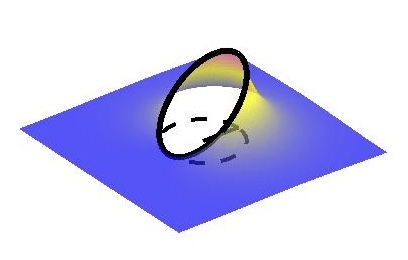
\includegraphics[width=0.2\textwidth]{LPA.jpg}
  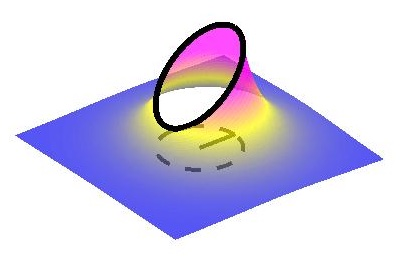
\includegraphics[width=0.2\textwidth]{LPB.jpg}
  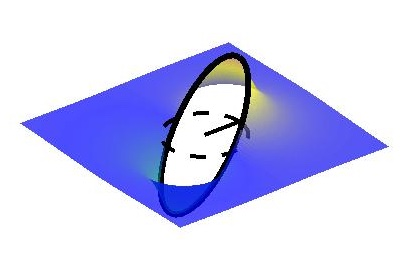
\includegraphics[width=0.2\textwidth]{LPC.jpg}
  \end{center}
  \vspace{-20pt}  
  \caption{\label{fig:bcs} Boundary conditions characterize the water
    structure at the particle interface: an amphiphilic particle (left),
    a hydrophobic
  particle with anisotropic intensity (middle), a water structure with
  positive/negative charge (right). The dashed curve is the boundary of the
  disk and the arrow is its director for each particle.}
\end{figure}


\begin{figure}
  \begin{center}
  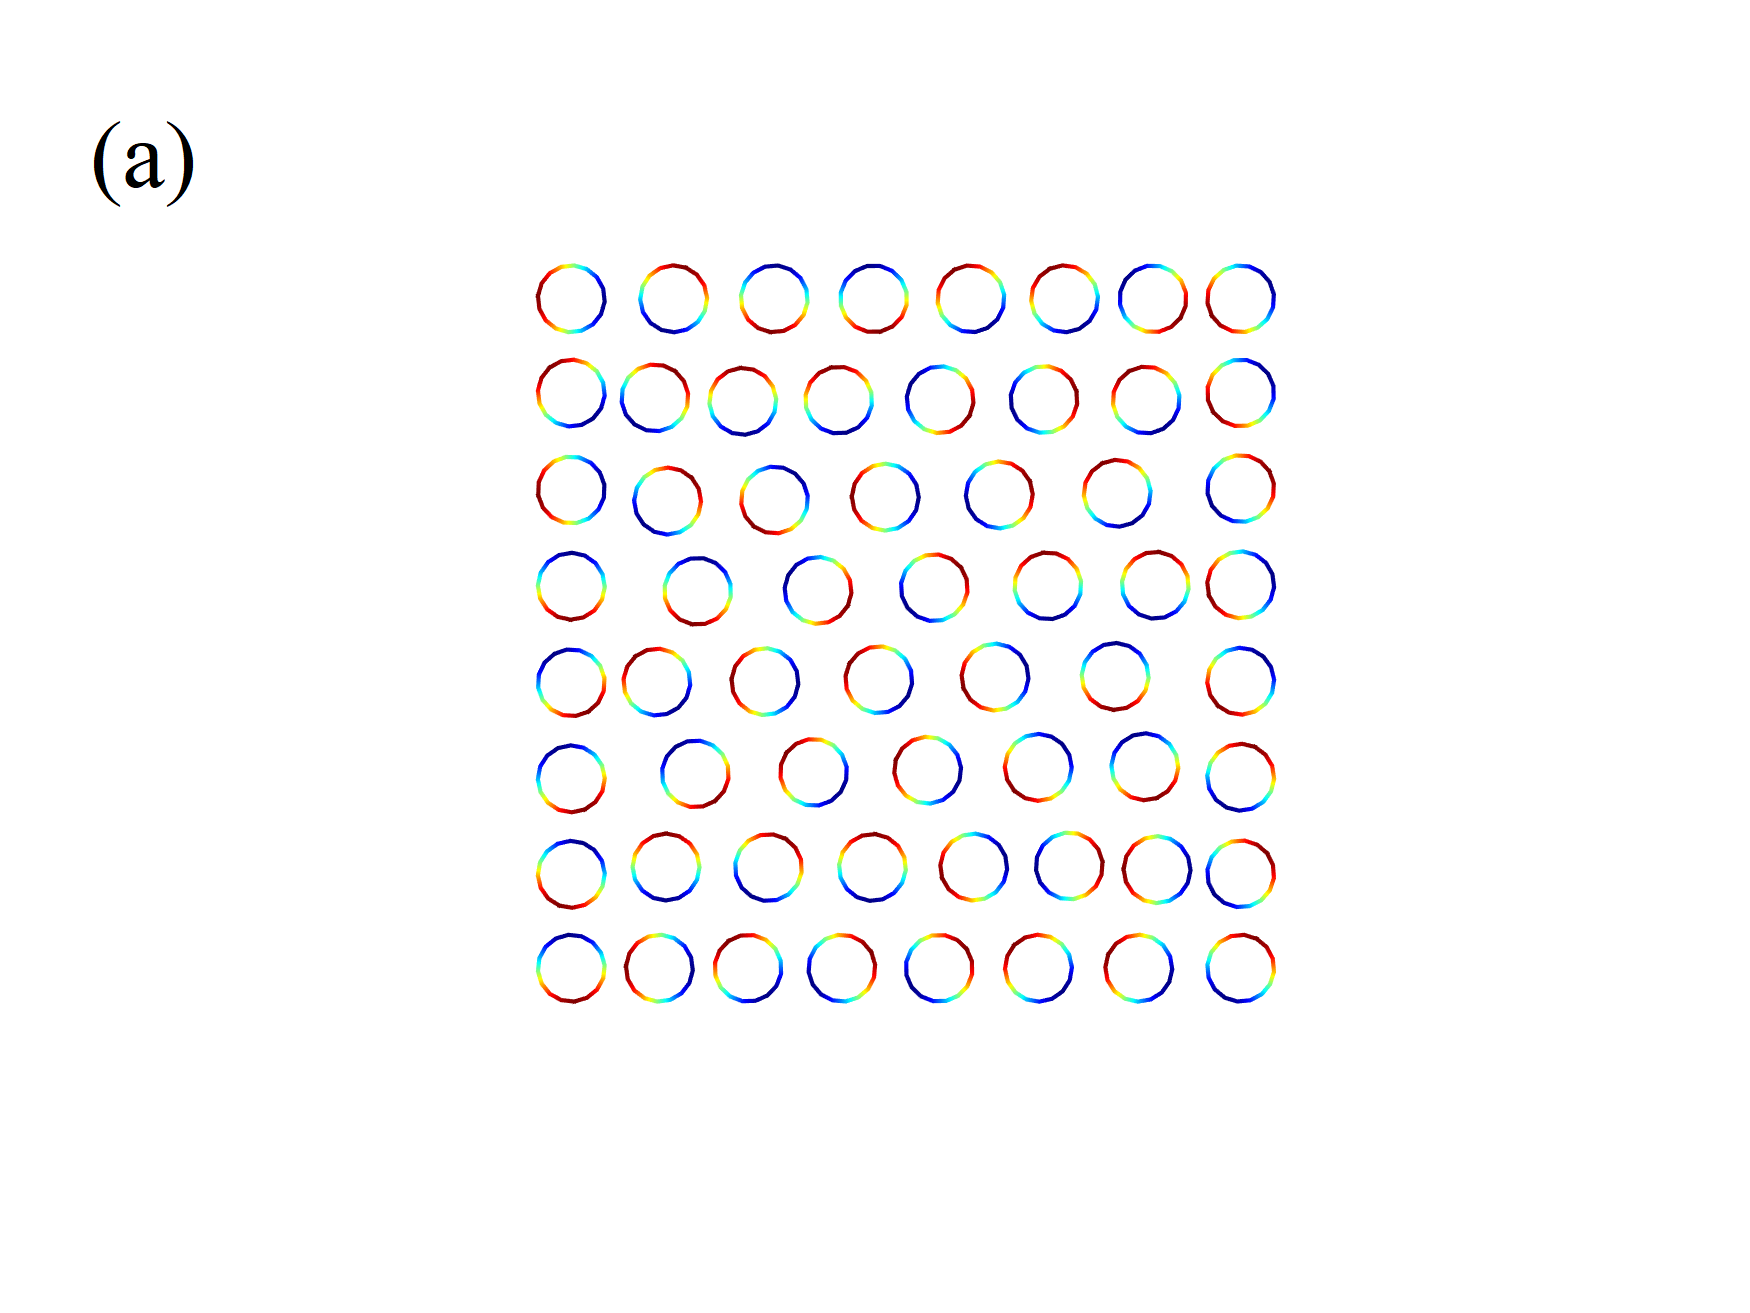
\includegraphics[width=0.4\textwidth]{Fig2a.png}
  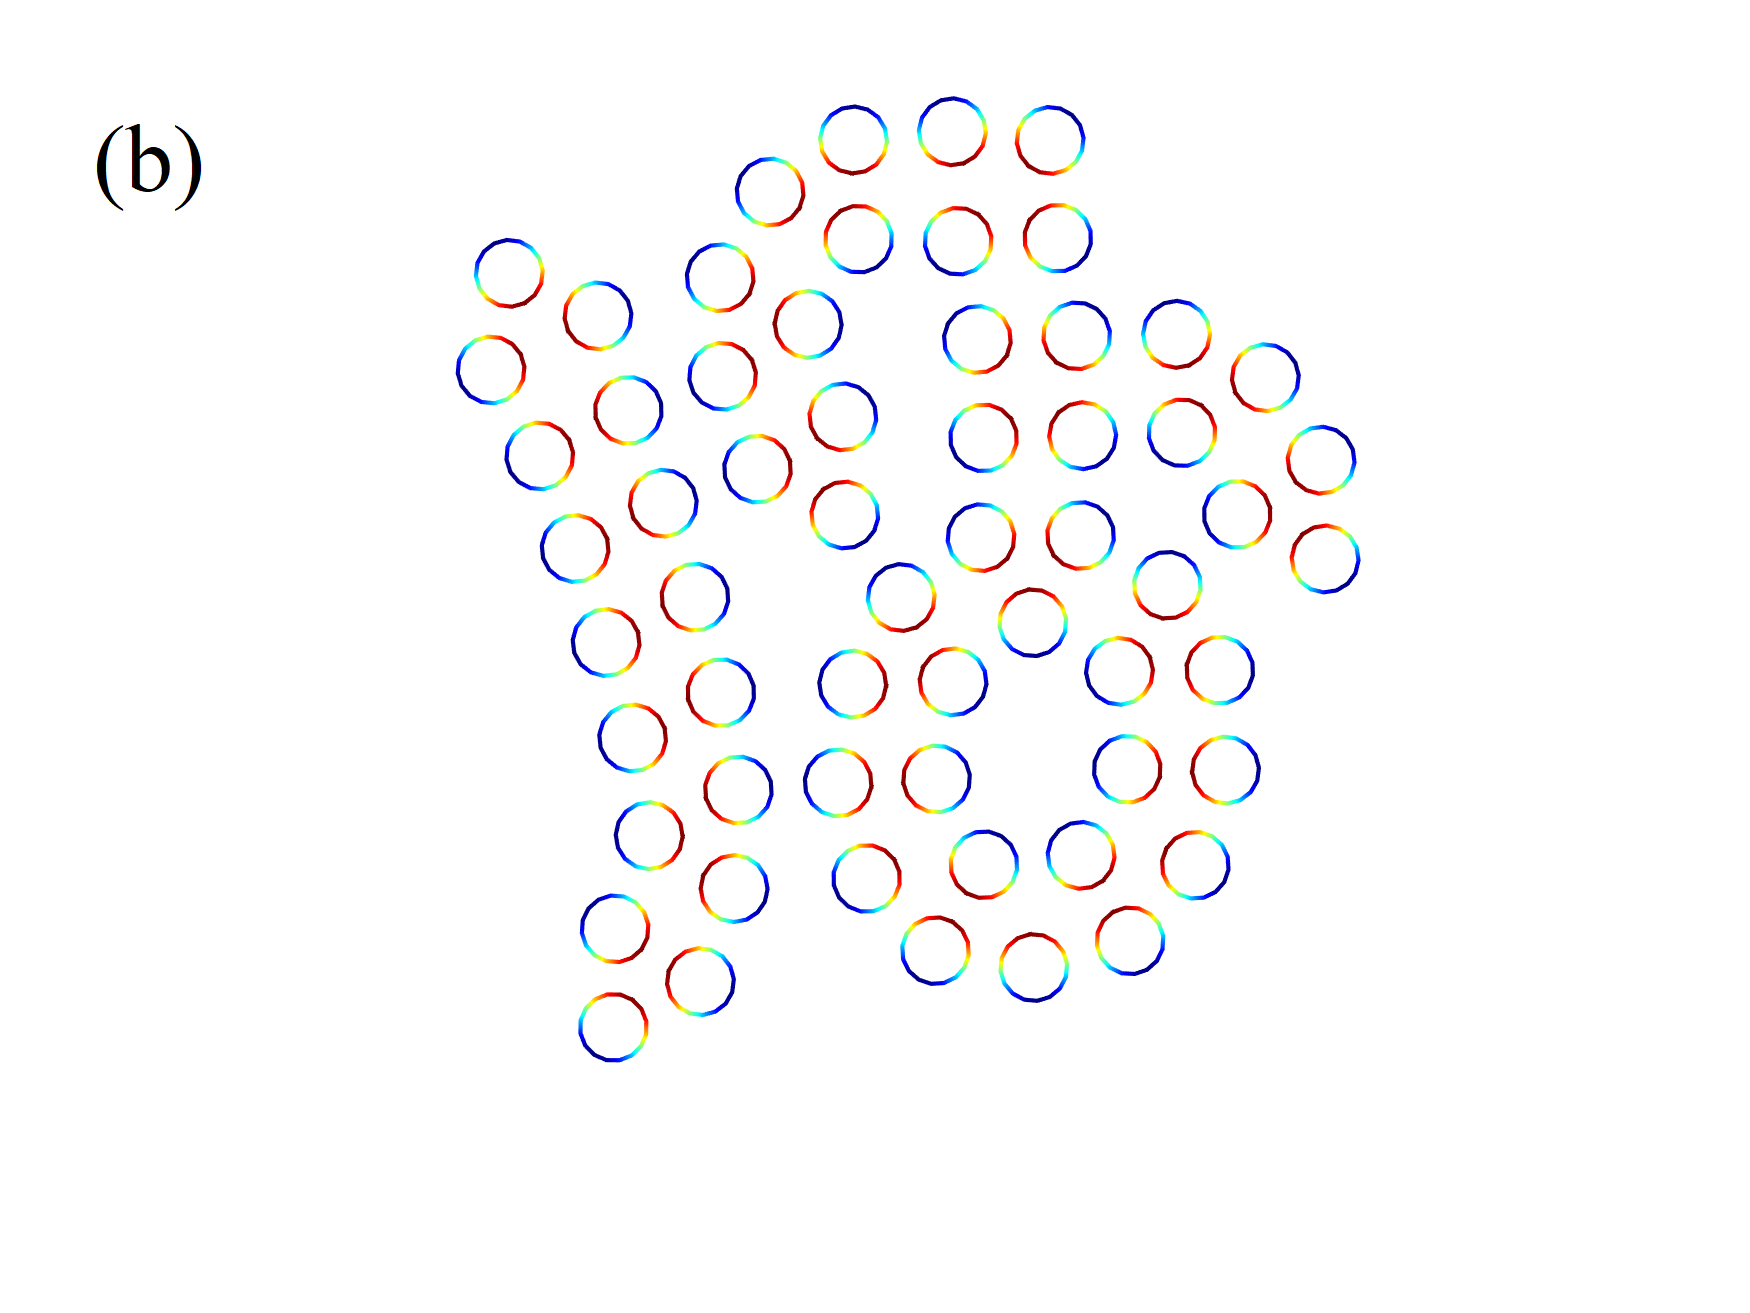
\includegraphics[width=0.4\textwidth]{Fig2b.png}\\
  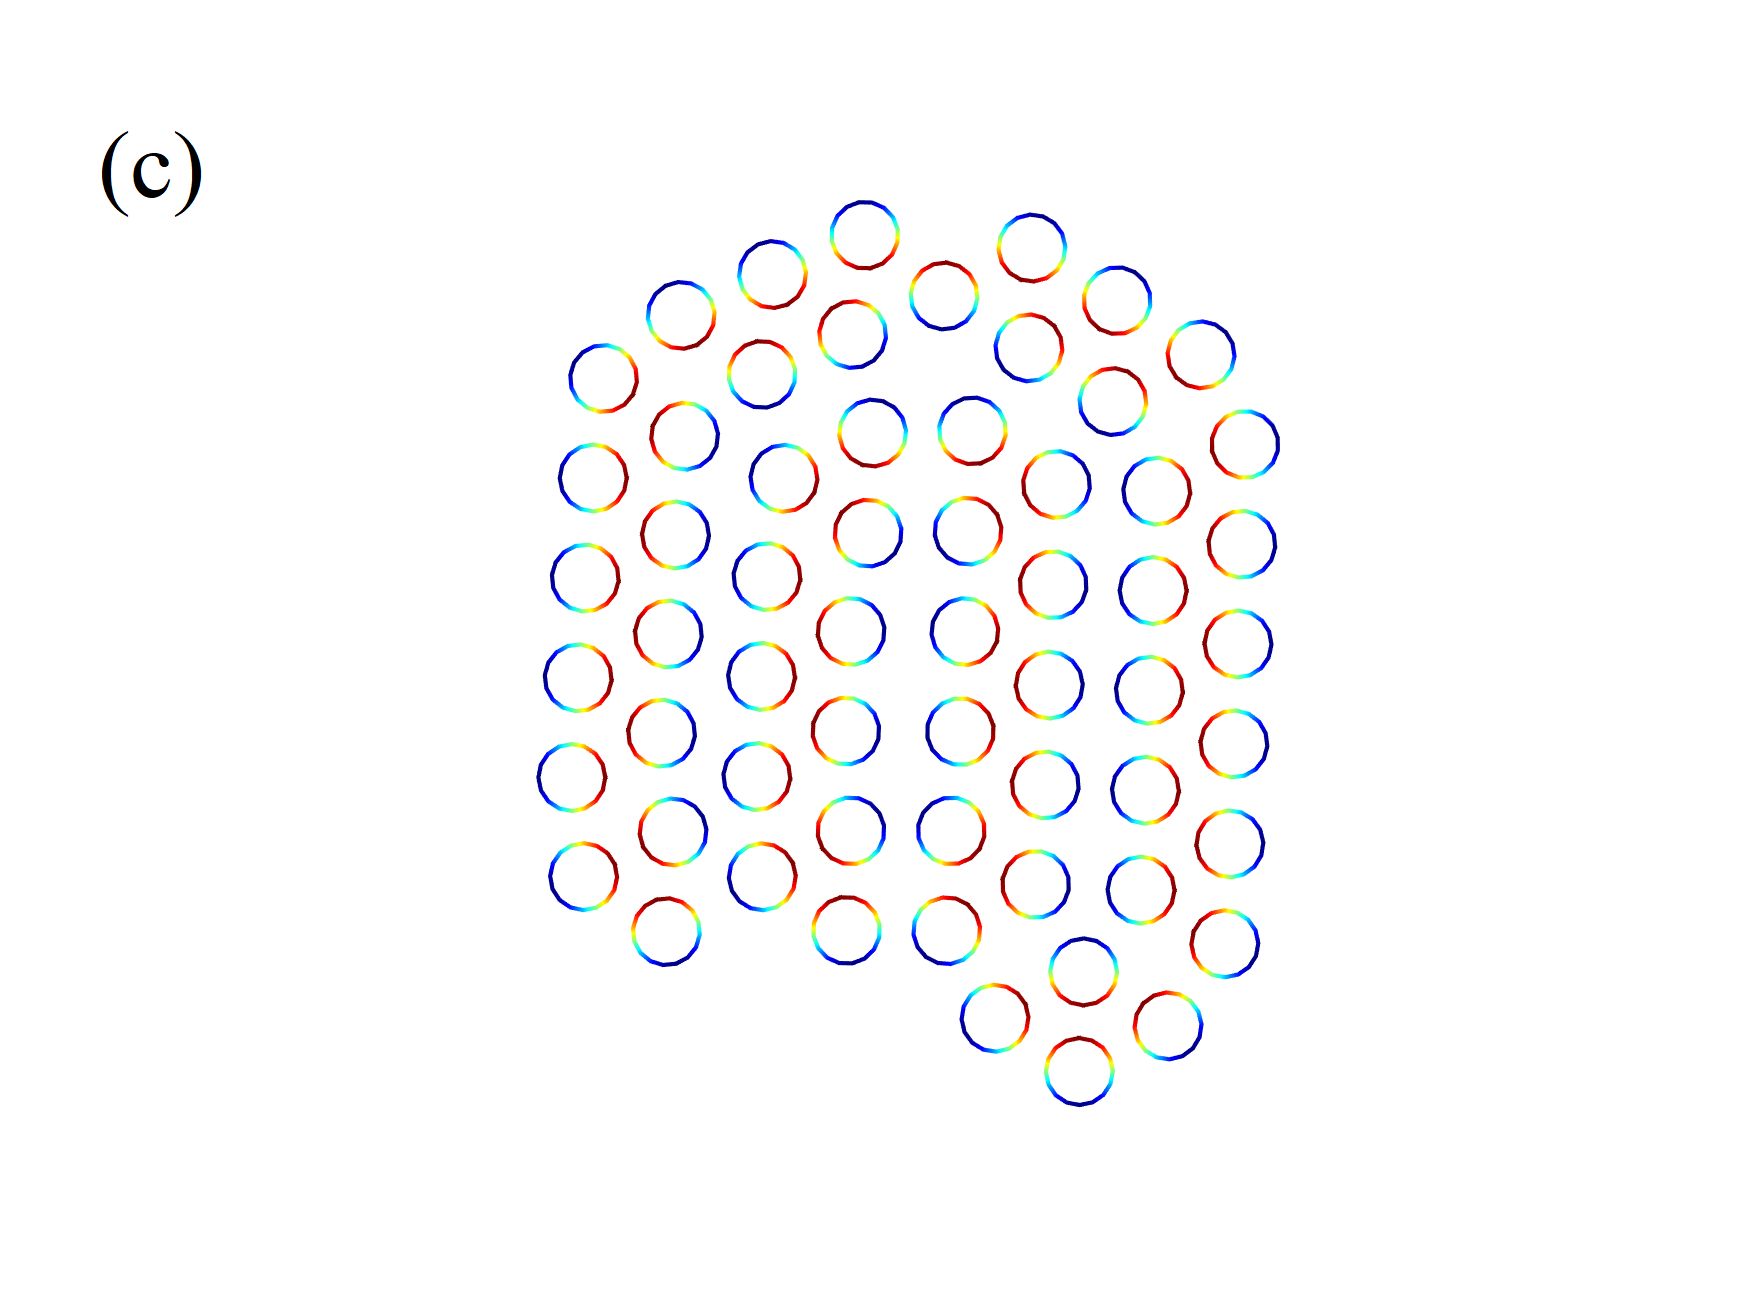
\includegraphics[width=0.4\textwidth]{Fig2c.png}
  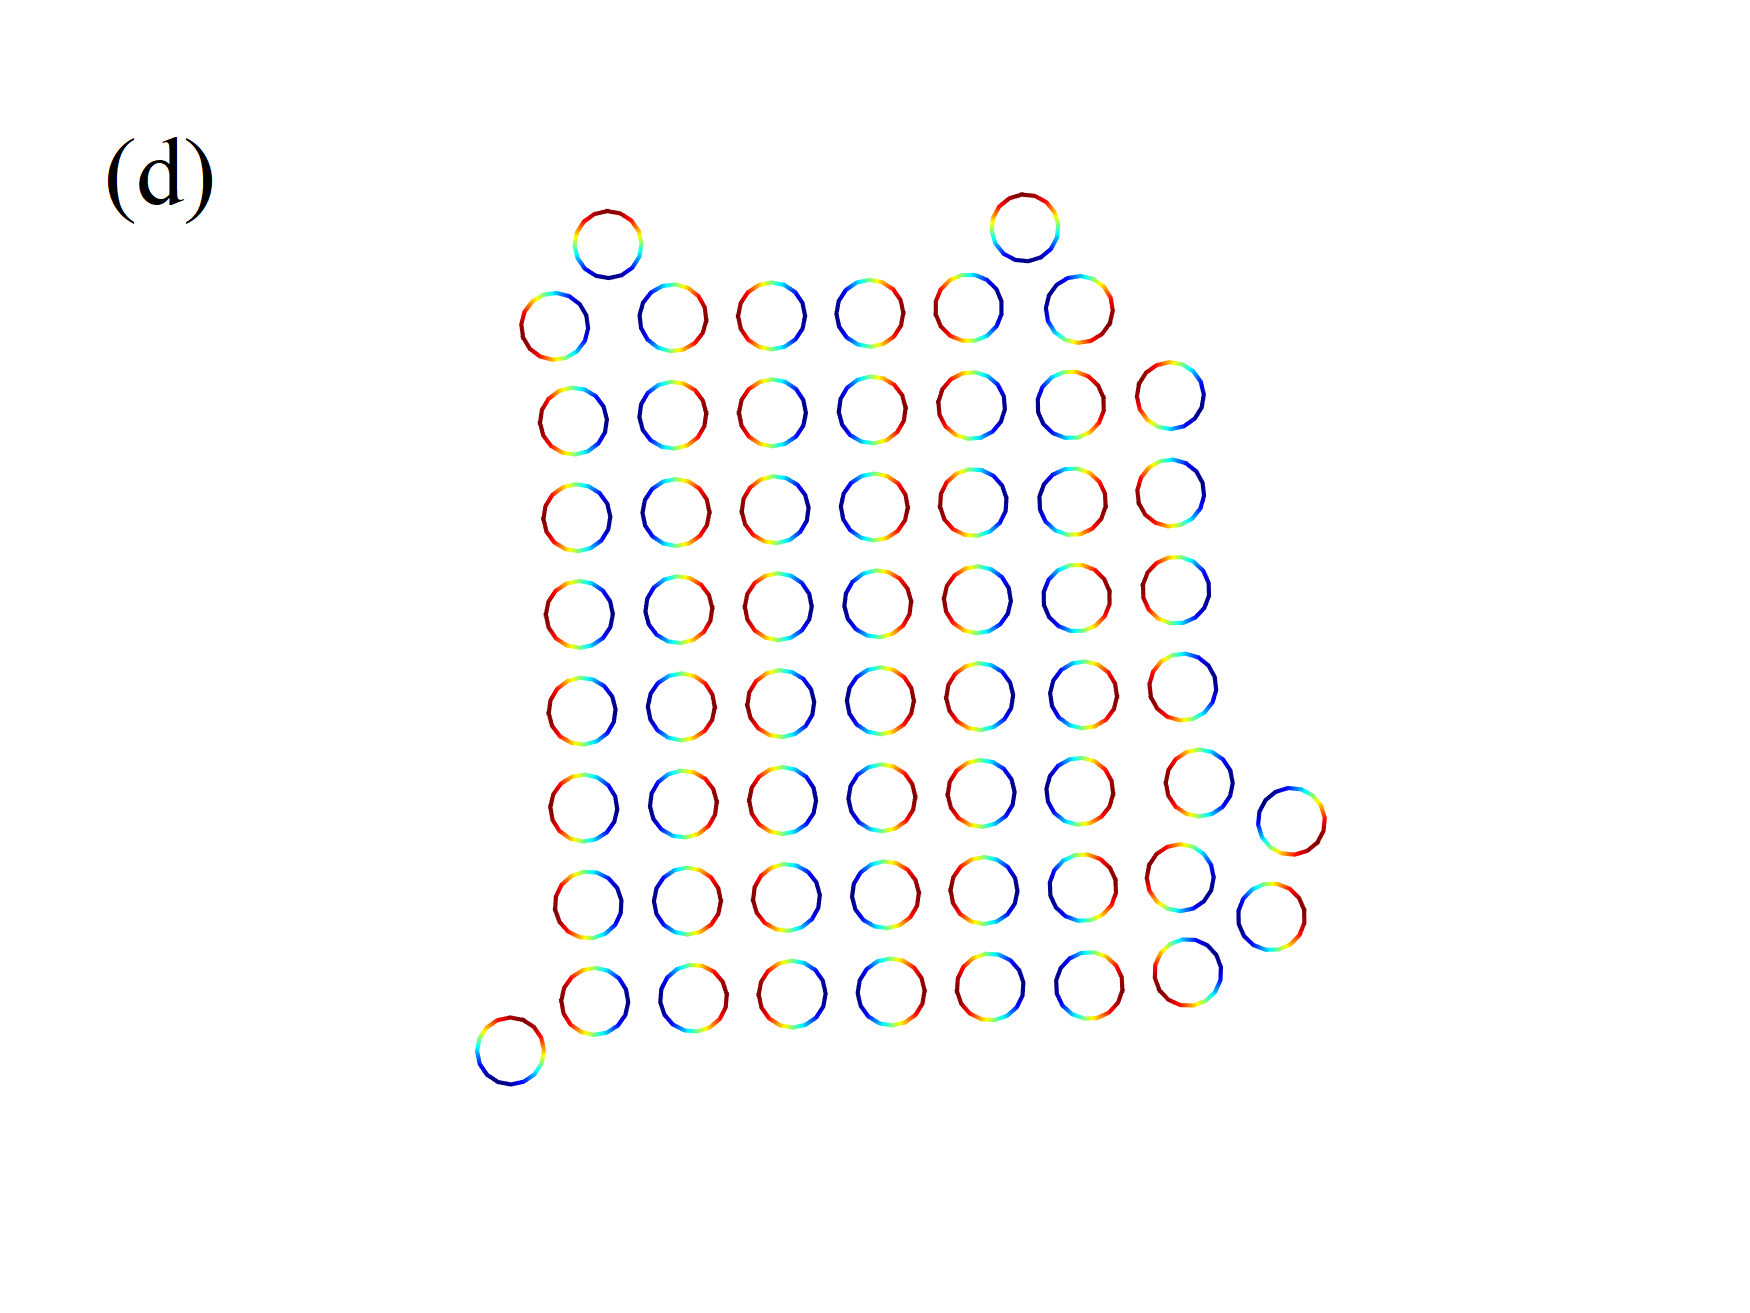
\includegraphics[width=0.4\textwidth]{Fig2d.png}
  \end{center}
  \vspace{-20pt}  
  \caption{\label{fig:relax} (a) Initial configuration for $N_b=60$ structure. In order to expedite the self-assembly procedure, all particles are placed in a $8\times8$ box initially. (b)--(d) Equilibruim states for all boundary conditions~\eqref{eq:bcs}(i)--(iii), respectively. Colors represent the boundary values that increases from minimum (blue) to maximum (red).  Panel (b) reaches the equilibrium at $t=1200$; Panel (c) reaches the steady-state at $t=600$; Panel (d) reaches the final state at $t=180$.}
\end{figure}


Case (i) models amphiphilic particles.
Amphiphilic particles have a hydrophobic tail and a hydrophilic head
and these are accounted for as follows.
The hydrophilic side takes the value $u =0$.
This mimicks the apolar head of a lipid, for example, which does
not alter the structure of adjacent waters. The hydrophobic side
represents hydrocarbons and takes the value 
$u > 0$. The interaction between particles is attractive,
and particles will collectively orient their tails toward
one another. Figure~\ref{fig:relax}(b) demonstrates multiple bilayer structures such as pancake and vesicle shapes.


Multilamelar bilayers arise when both sides of the particle 
are hydrophobic. 
The boundary condition \eqref{eq:bcs}(ii) 
gives a particle with a hydrophobic intensity that is greater
on the $\theta_i = 0$ side than on the $\theta_i = \pi$ side.
The initial self-assembly is similar to that in case (i).
The difference arises in the long-time dynamics where the bilayers
no longer remain well-separated. 
Rather, the bilayers form layers 
as a consequence of the interfacial tension of exposed particle
heads.%~\cite{Huetal19, deMeetal21}. 
Figure~\ref{fig:relax}(c) shows the multilamellar structure with 8 layers when $N_b=60$. 
The number of folds depends on several factors, for instances, number of particles and intial configurations.


Finally, boundary condition \eqref{eq:bcs}(iii) models 
a particle whose head surface repels the tail surface as proposed in
\cite{MaRa76, Ma77}.
The particles initially form chains with their directors perpendicular to the
length of the chain. The equilibrium structure
resembles a checkerboard pattern
where each particle coordinates
its head with the head of three other particles and its tail with the
tail of three other particles. % Figure~\ref{fig:self-assembly}(c).
Figure~\ref{fig:relax}(d) gives an example that this boundary condition results a checker board/stripes equilibrium state.


\subsection{Collective Janus Particles Suspended in a Shear Flow}
%%%


Consider placing equilibrium states of boundary condition \eqref{eq:bcs} (ii) for 60 particles in a shear flow,
\begin{equation}
\uu_\infty(\xx) = \dot\gamma ({\bf e}_y\cdot\xx){\bf e}_x,
\end{equation}
%
where $\dot\gamma$ is the shear rate. Figure~\ref{fig:shear_1} (a)--(c) show the snapshots of simulation results when $\dot\gamma=0.05$.
We measure the ratio of major and minor axes $\lambda$ by adopting an ellipse fitting using the singular value decomposition and track the ratio of this multi-lamellar structure when the flow is on. 
The result is shown in panel (d) and we observe that the multi-lamellar structure will be stretched 
to a pancake shape while the ratio reaches above $\lambda=3.5$ level.

Notice that for this simulation, the center of mass position of the initial configuration is not at the origin and it is slightly to the right of the origin. Therefore, the result has shown that the structure stretching occurs earlier that the case when we shift the center of mass position to the origin. 

\begin{figure}
  \begin{center}
  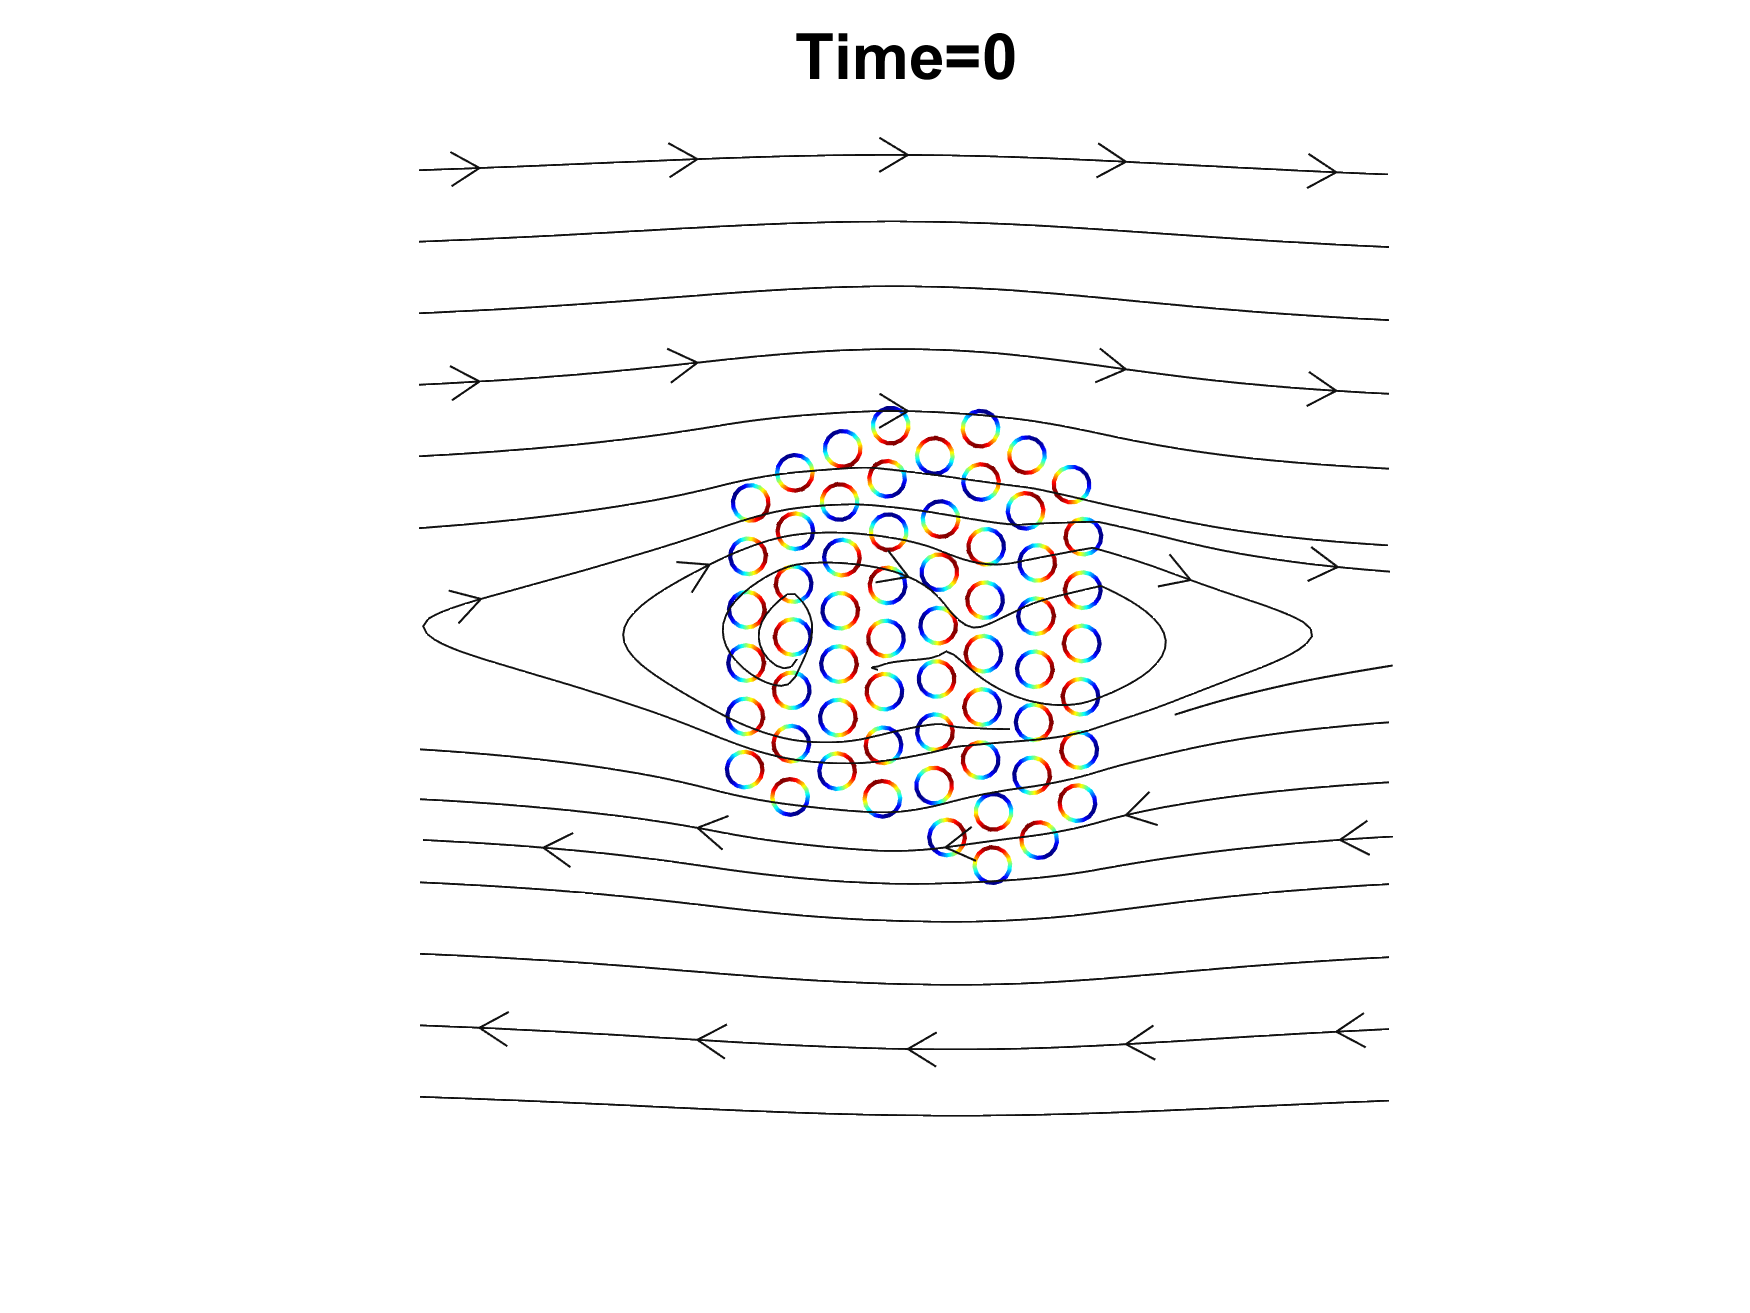
\includegraphics[width=0.4\textwidth]{shear_0.png}
  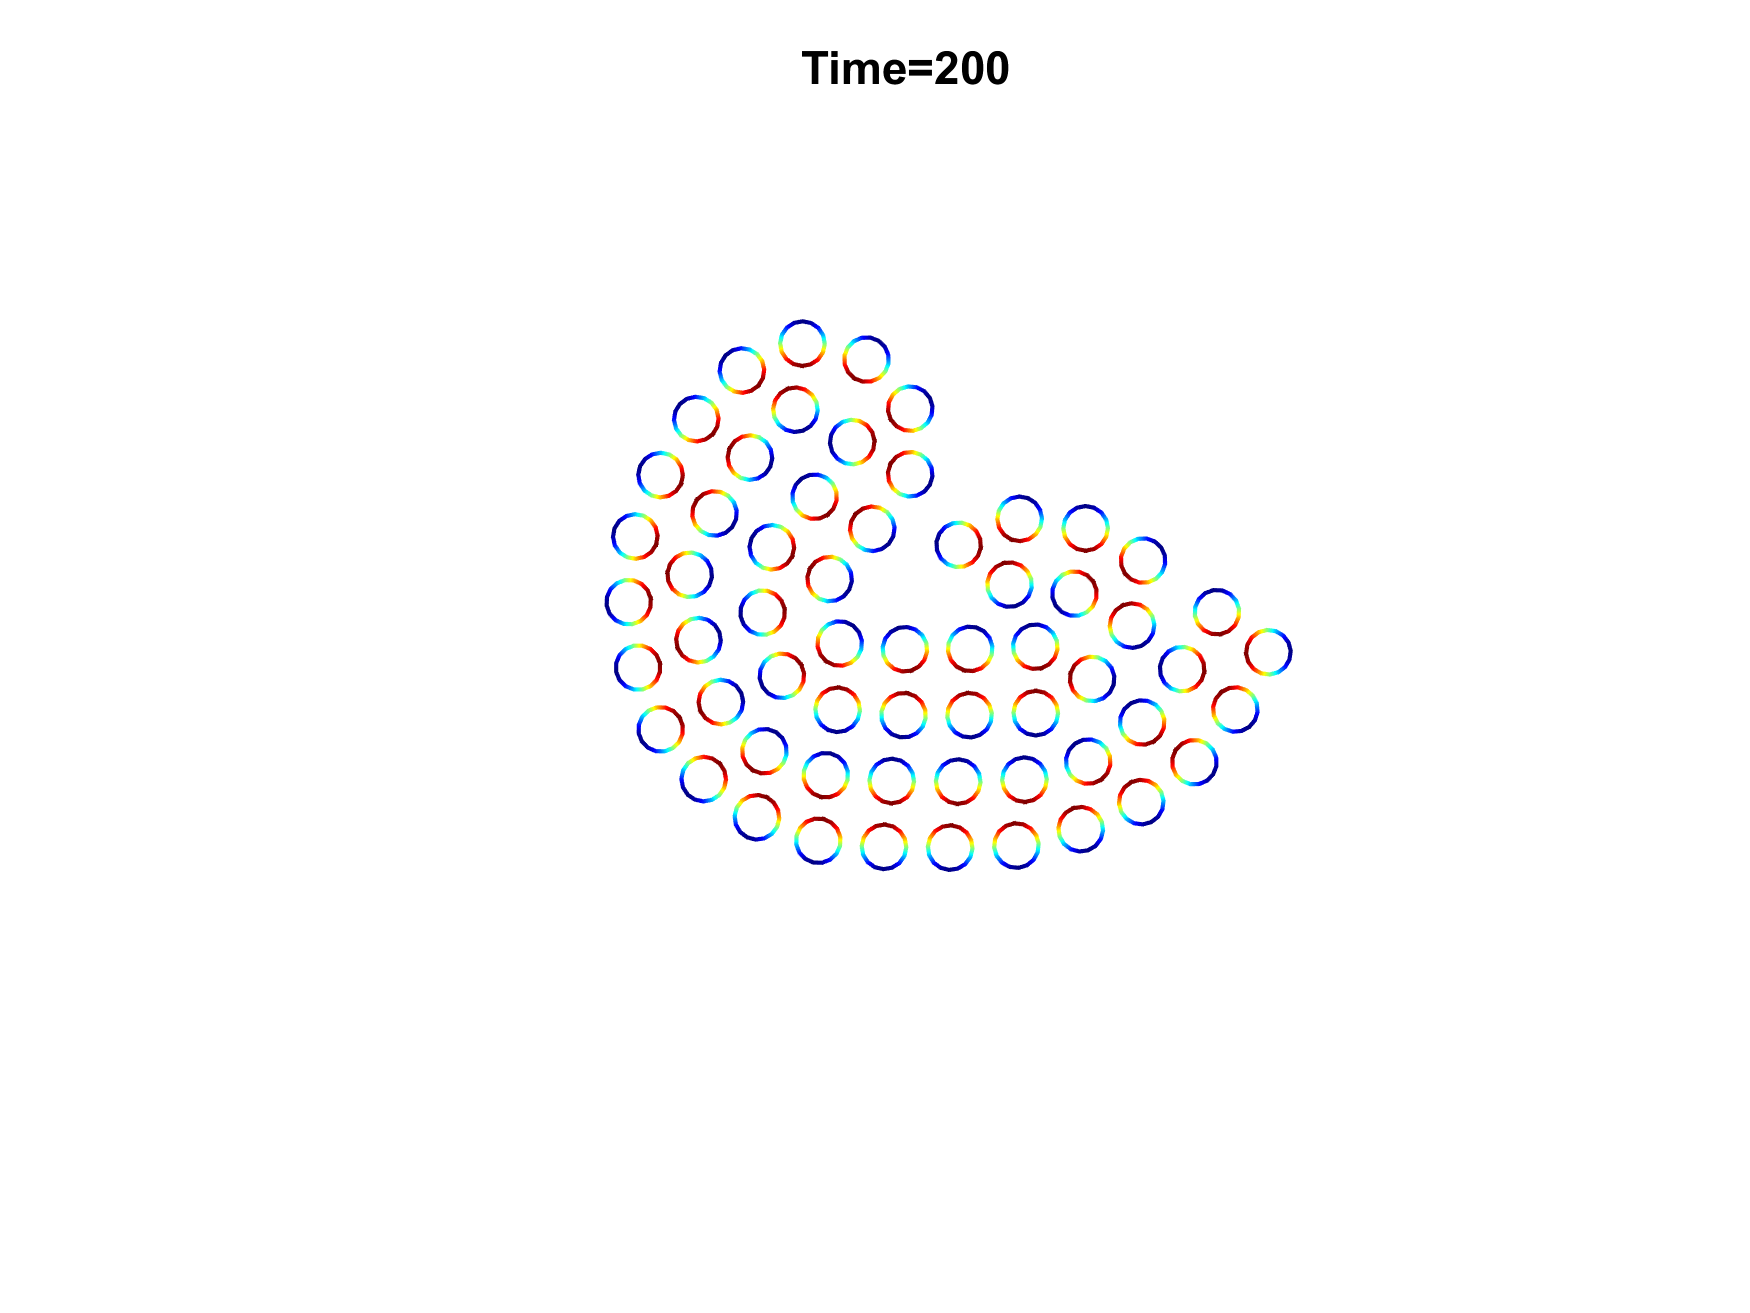
\includegraphics[width=0.4\textwidth]{shear_1000.png}\\
  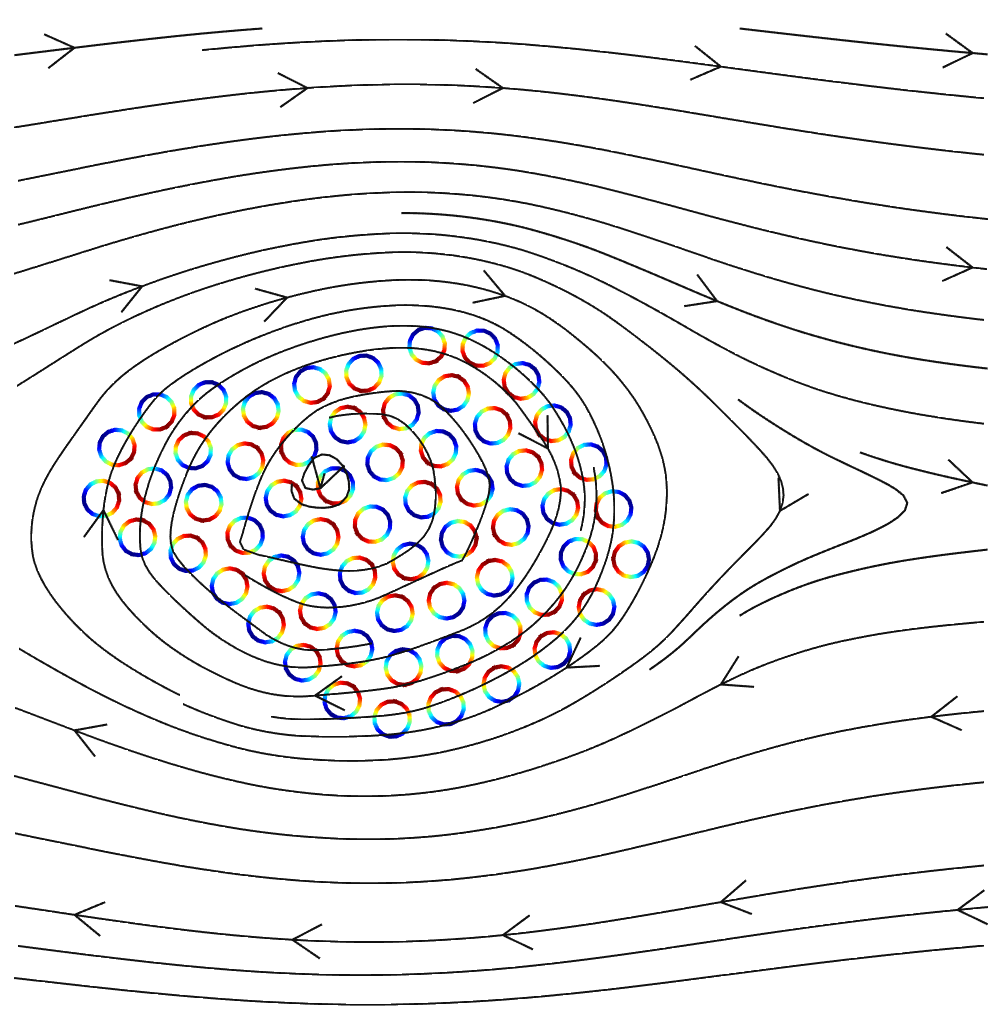
\includegraphics[width=0.4\textwidth]{shear_2000.png}
    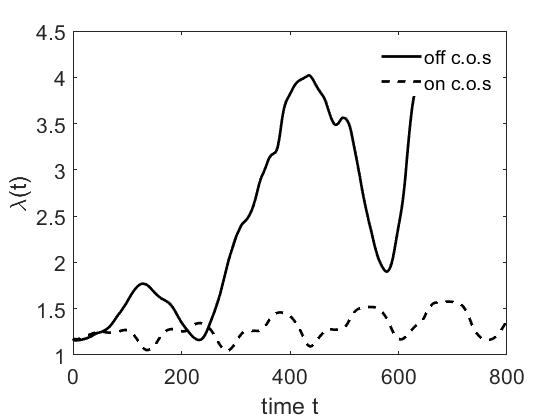
\includegraphics[width=0.4\textwidth]{shear_dist_all.jpg}
  \end{center}
  \vspace{-20pt}  
  \caption{\label{fig:shear_1} Snapshots of simulation using boundary condition \eqref{eq:bcs}(ii) in a shear flow when $\dot\gamma=0.05$. }
\end{figure}

%%%

The second set of simulation is putting the equilibrium state of the boundary condition \eqref{eq:bcs} (iii), the checker board, in a shear flow. After a set of empirical numerical investigations, we obtain a critical shear rate $\dot\gamma=0.15$ where the checker board deforms into stripes and small groups of JP. Figure~\ref{fig:shear_2}(a)--(d) show configurations when $t=\{0,50,100,150\}$. %The deformation starts with stripe separations




\begin{figure}
  \begin{center}
  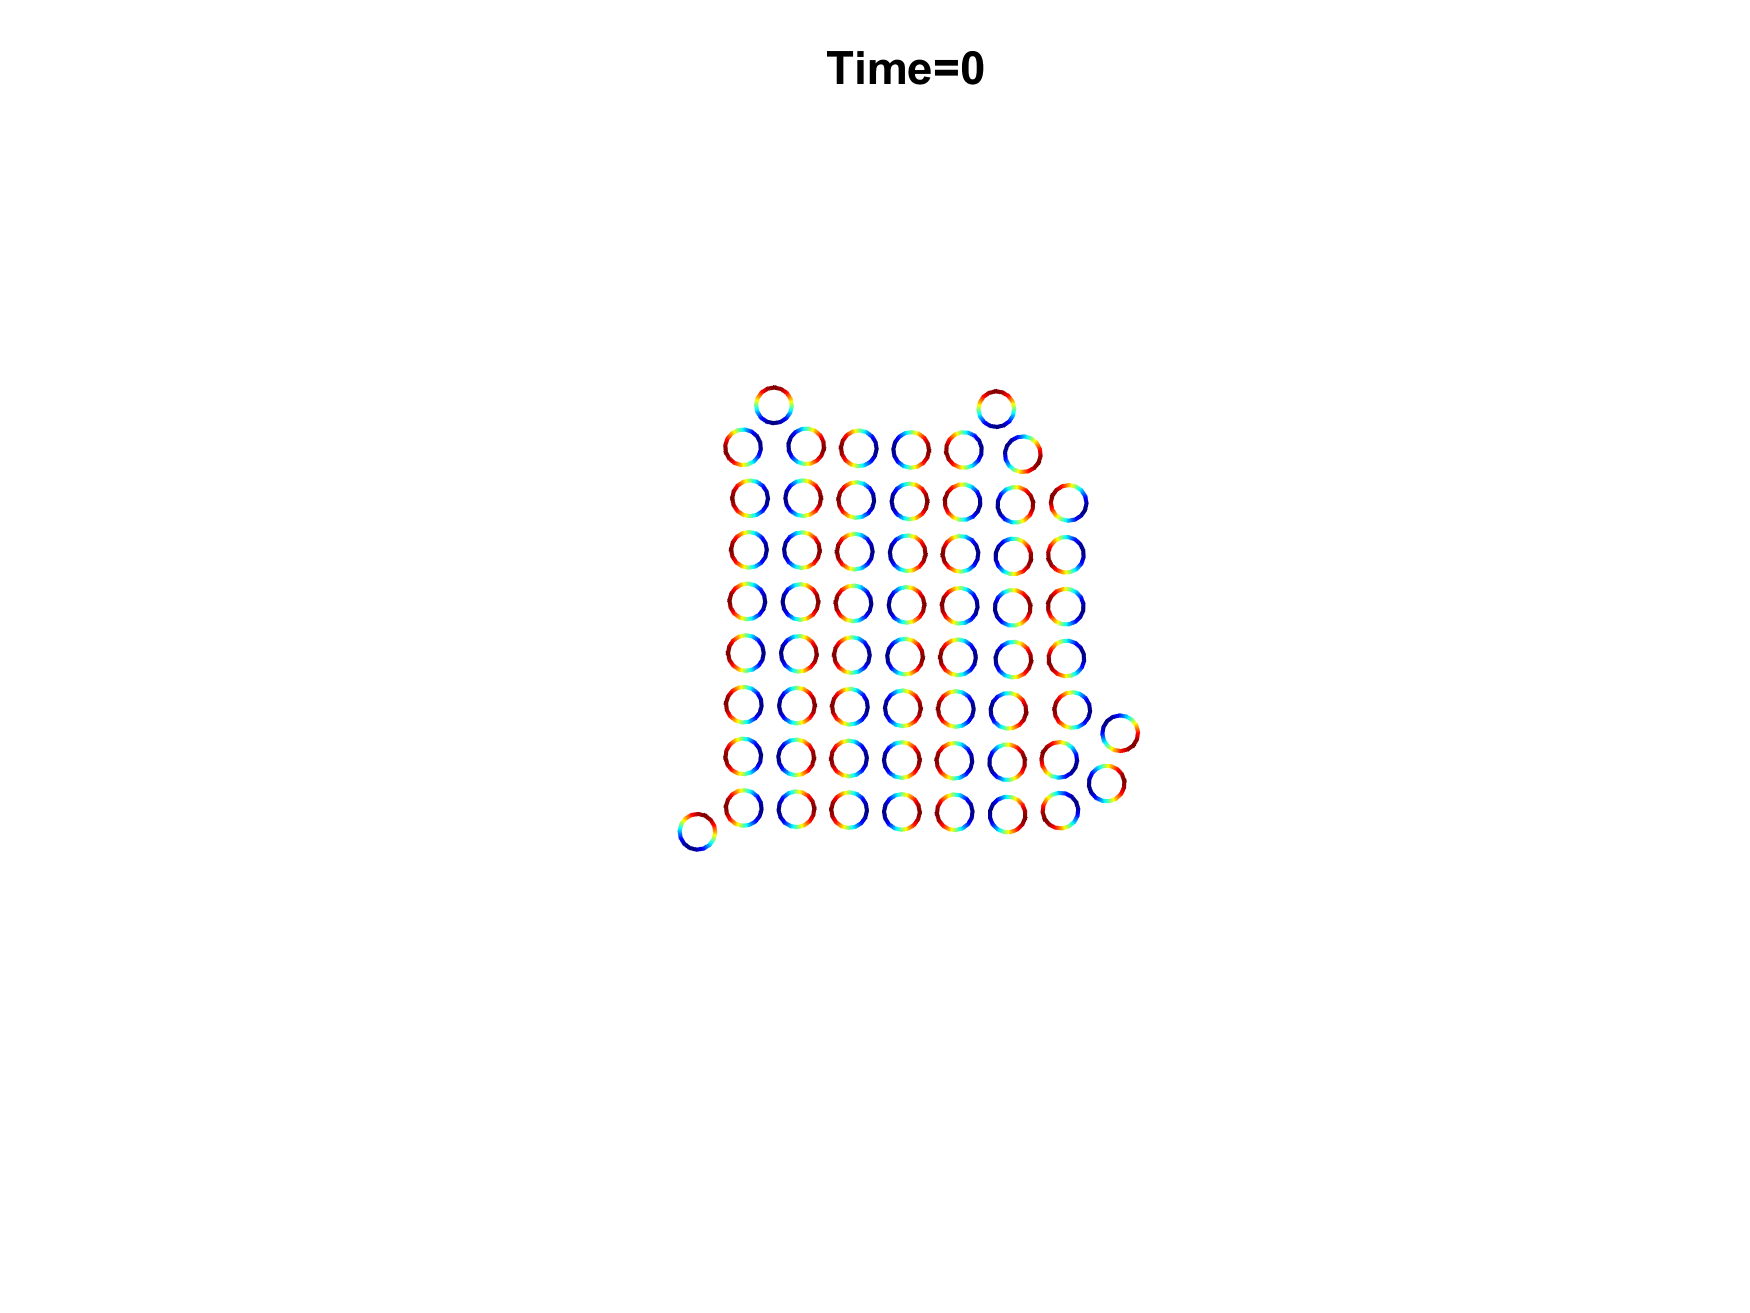
\includegraphics[width=0.4\textwidth]{shear_checker_0.png}
  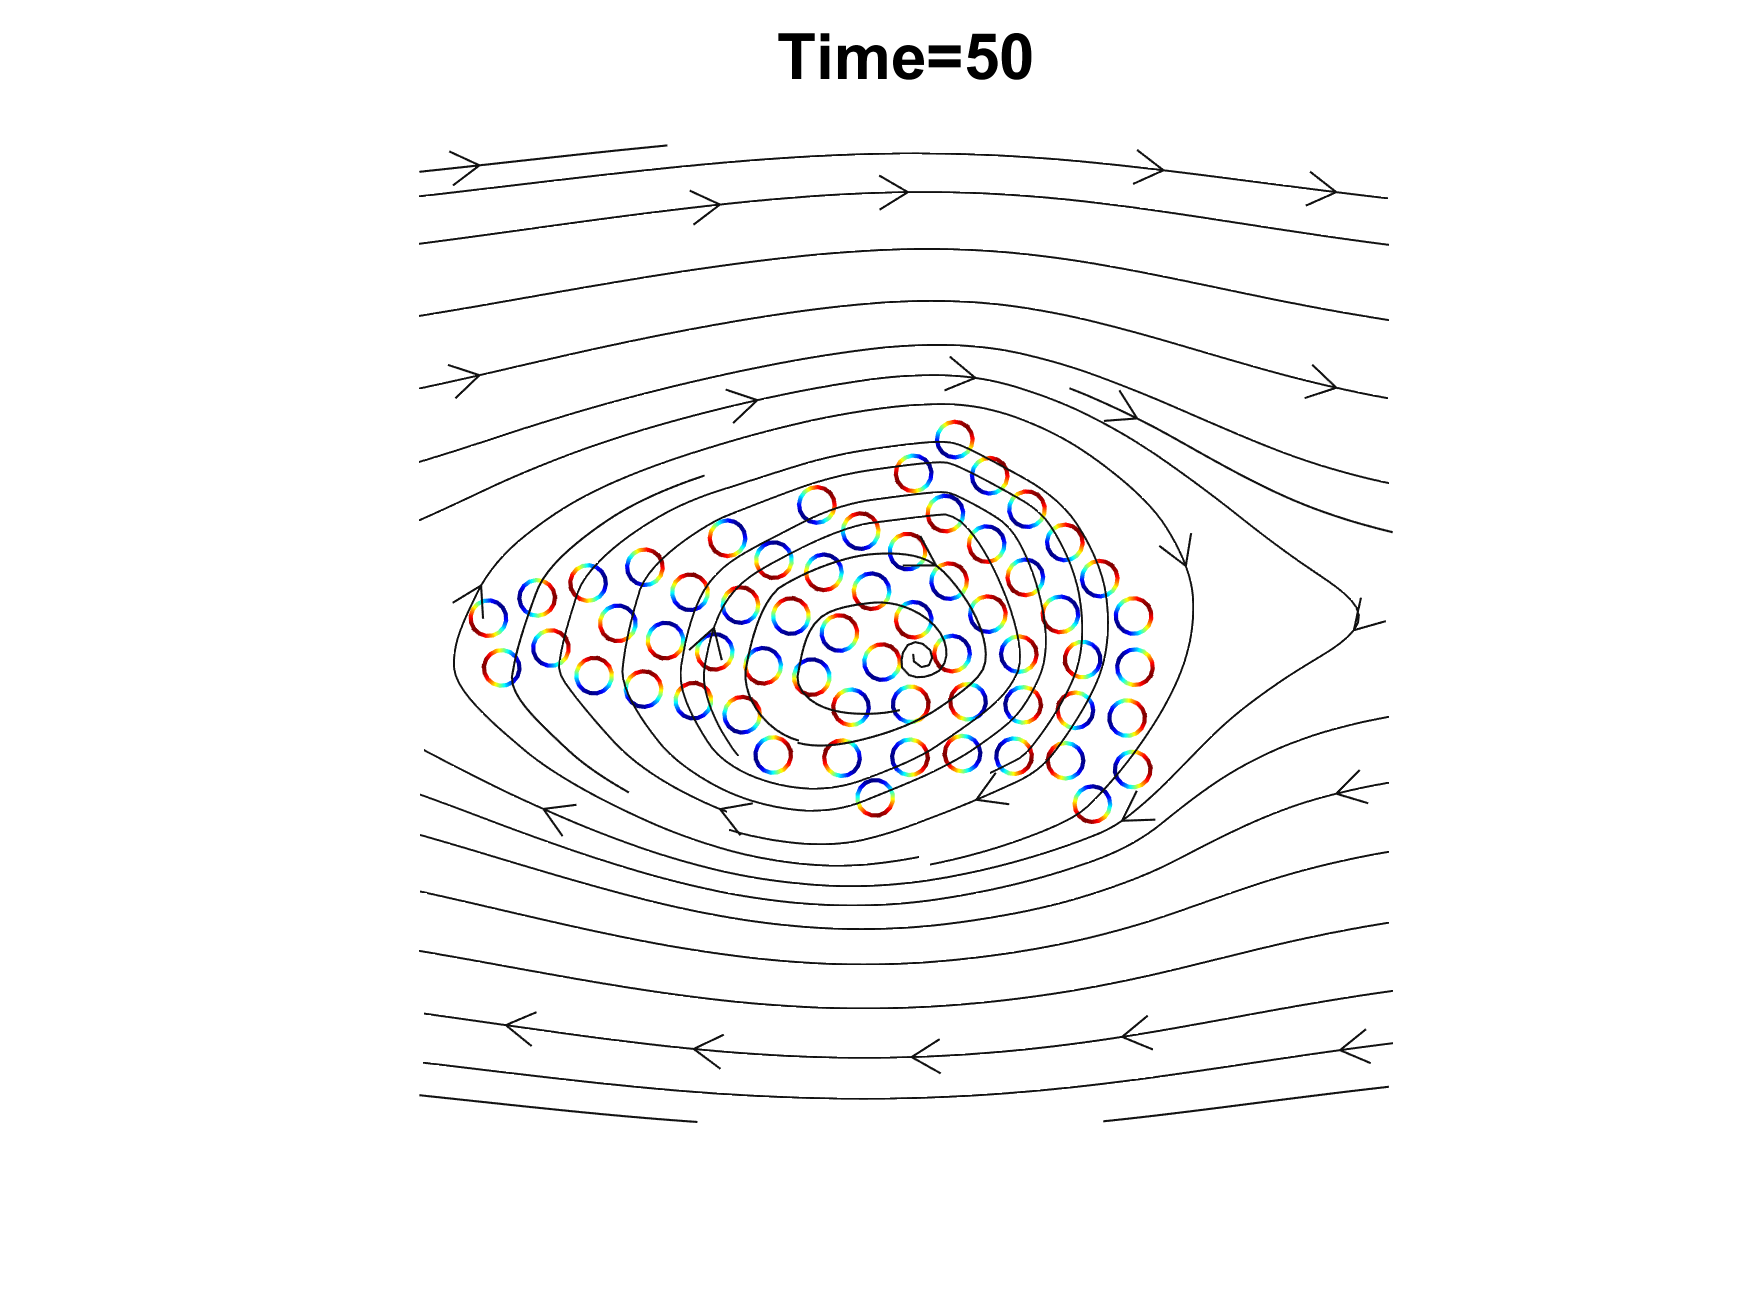
\includegraphics[width=0.4\textwidth]{shear_checker_250.png}\\
  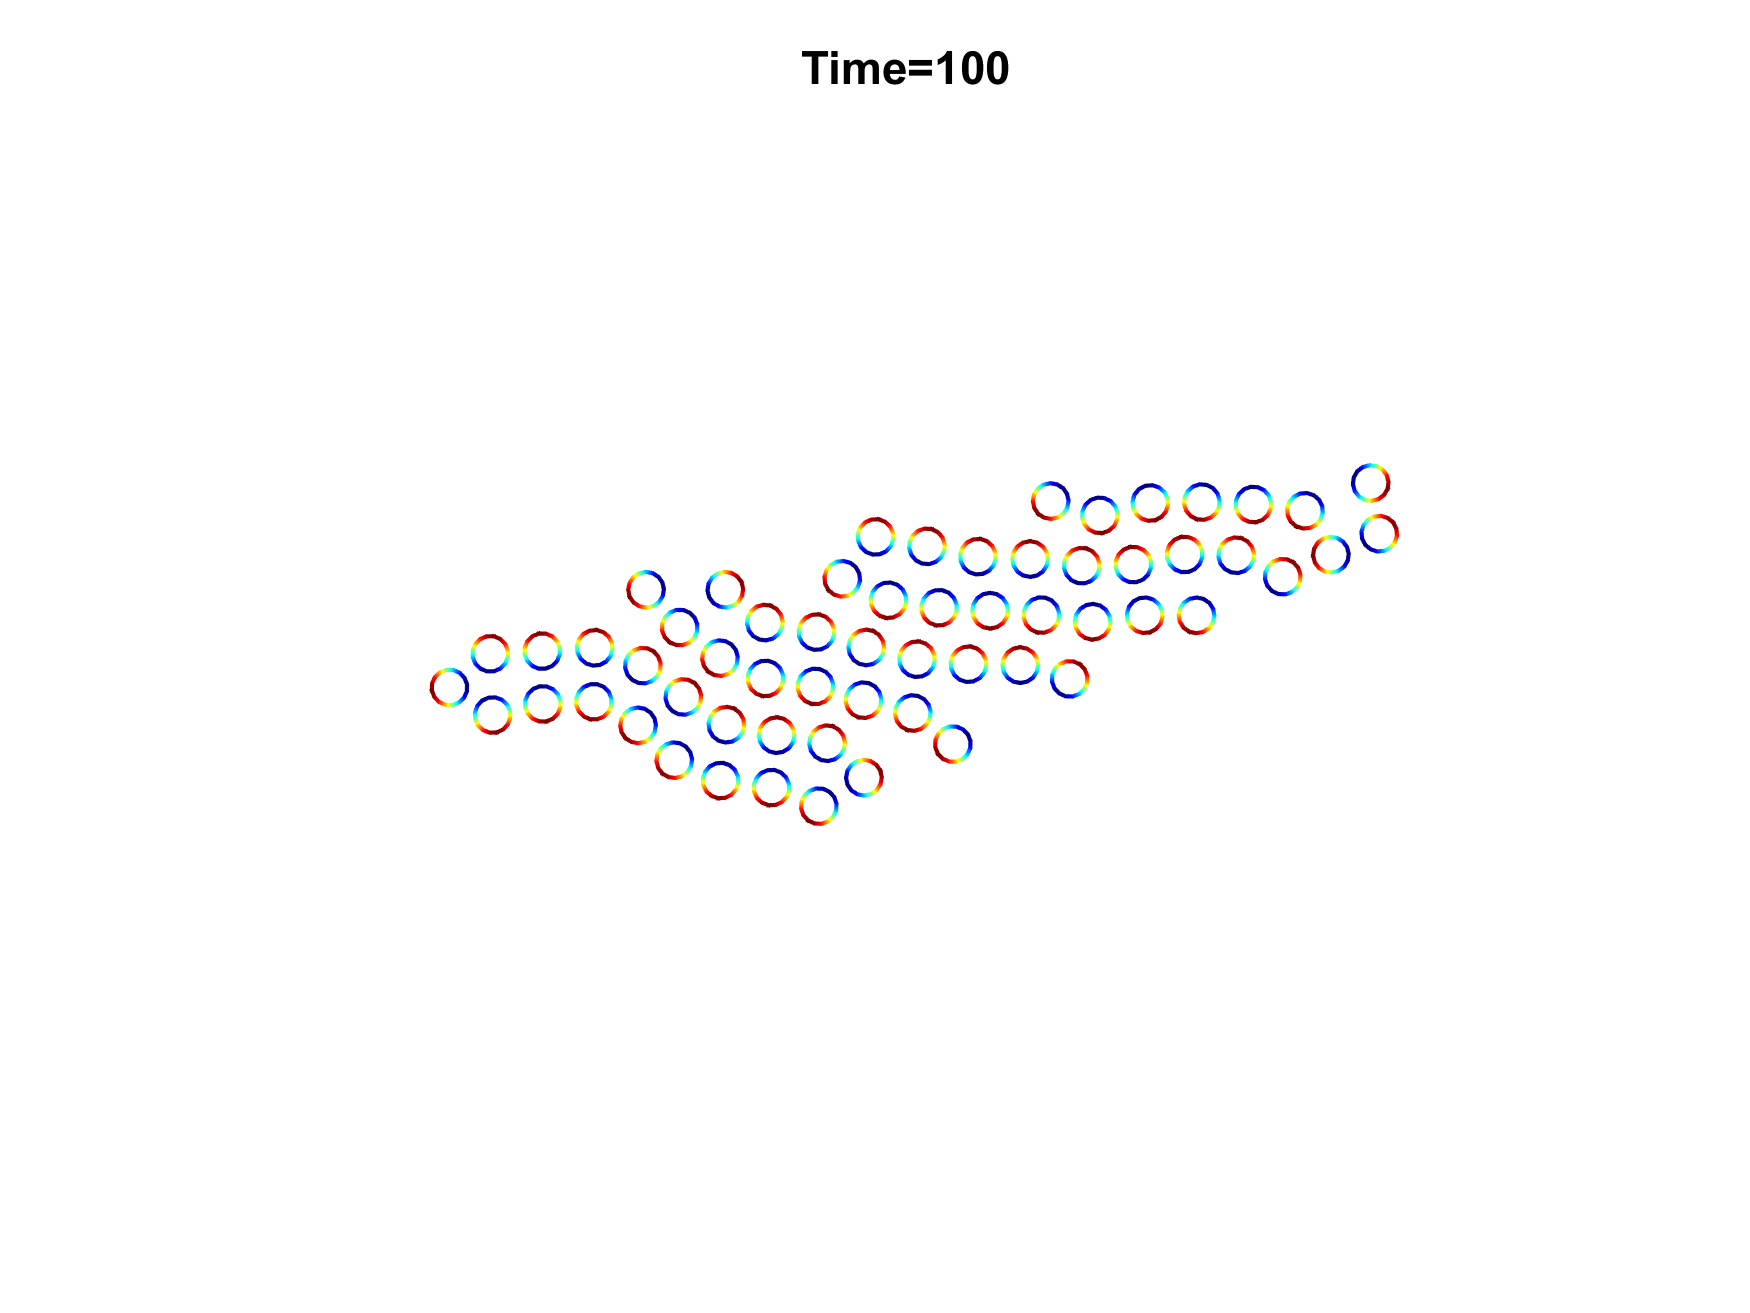
\includegraphics[width=0.4\textwidth]{shear_checker_500.png}
    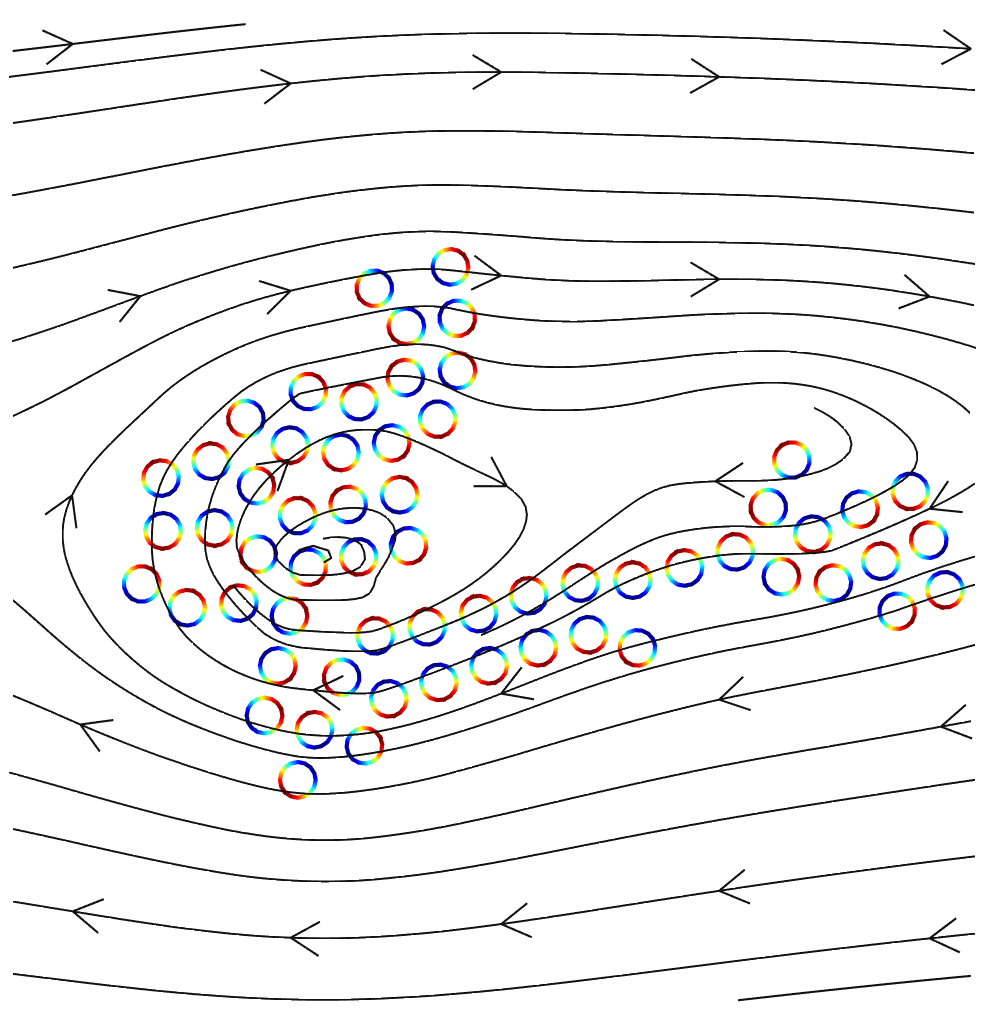
\includegraphics[width=0.4\textwidth]{shear_checker_750.png}
  \end{center}
  \vspace{-20pt}  
  \caption{\label{fig:shear_2} Snapshots of simulation using boundary condition \eqref{eq:bcs}(c) in a shear flow when $\dot\gamma=0.15$. }
\end{figure}


\subsection{Collective Janus Particles Suspended in a Taylor-Green Flow}

\begin{figure}
  \begin{center}
  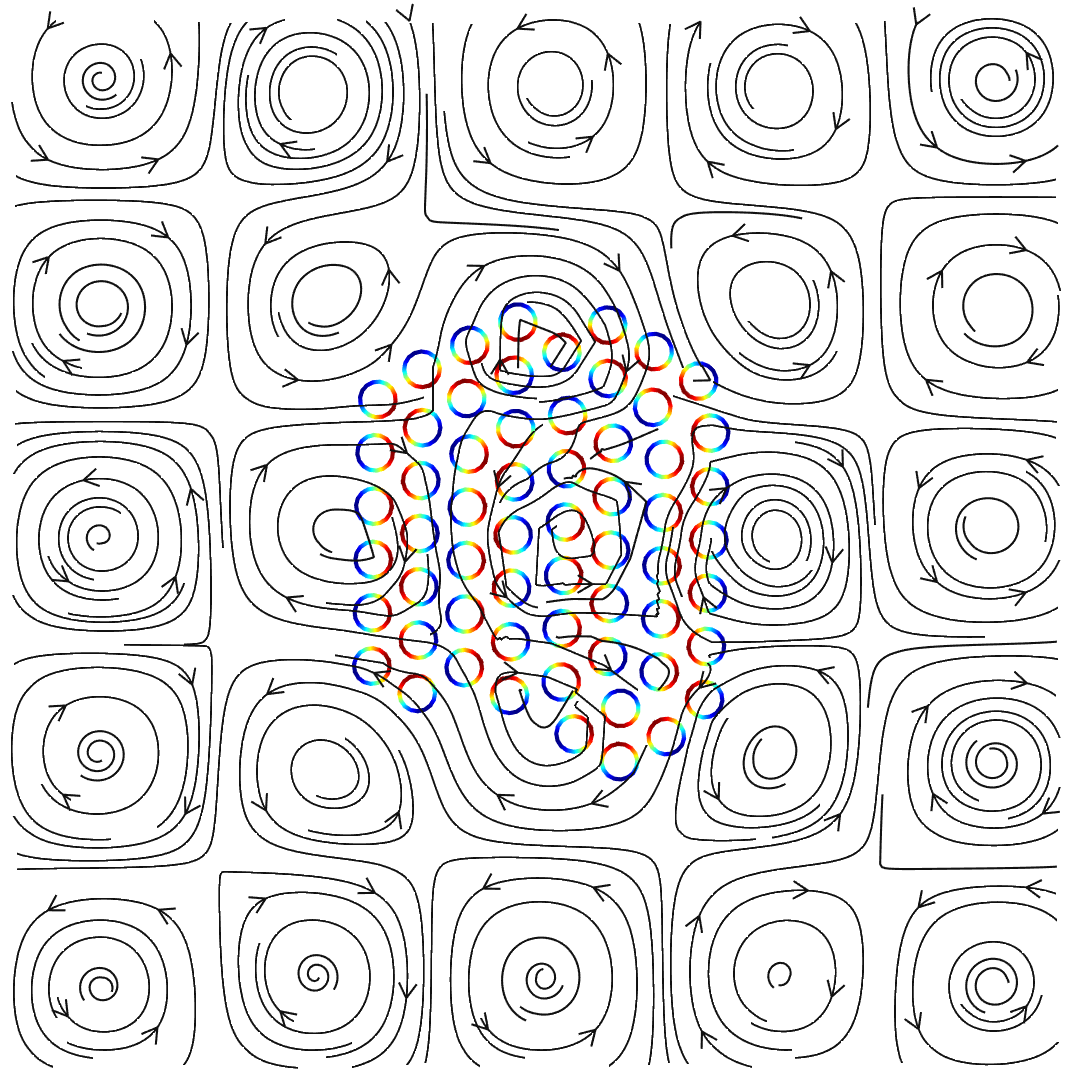
\includegraphics[width=0.4\textwidth]{TG_0.png}
  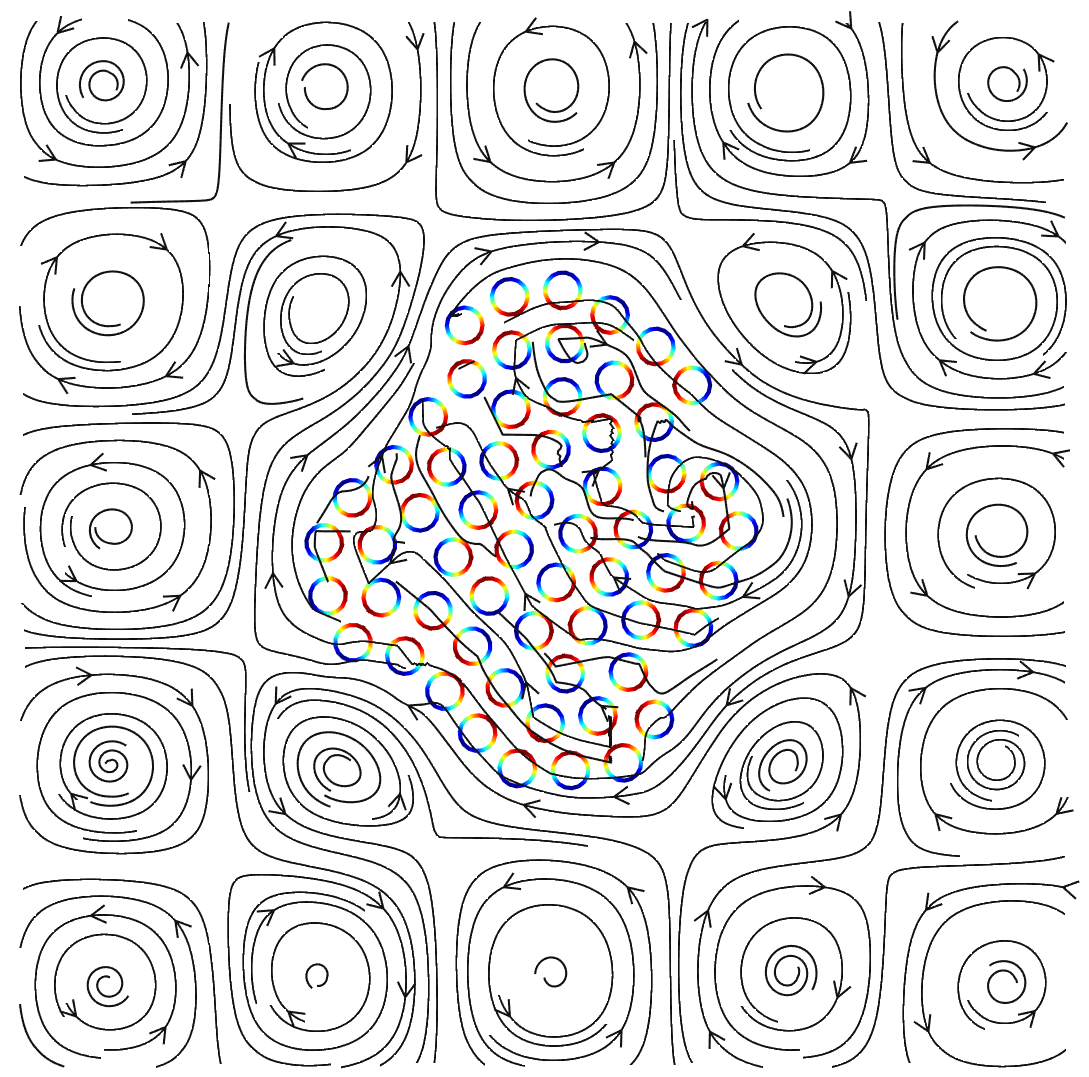
\includegraphics[width=0.4\textwidth]{TG_2500.png}\\
  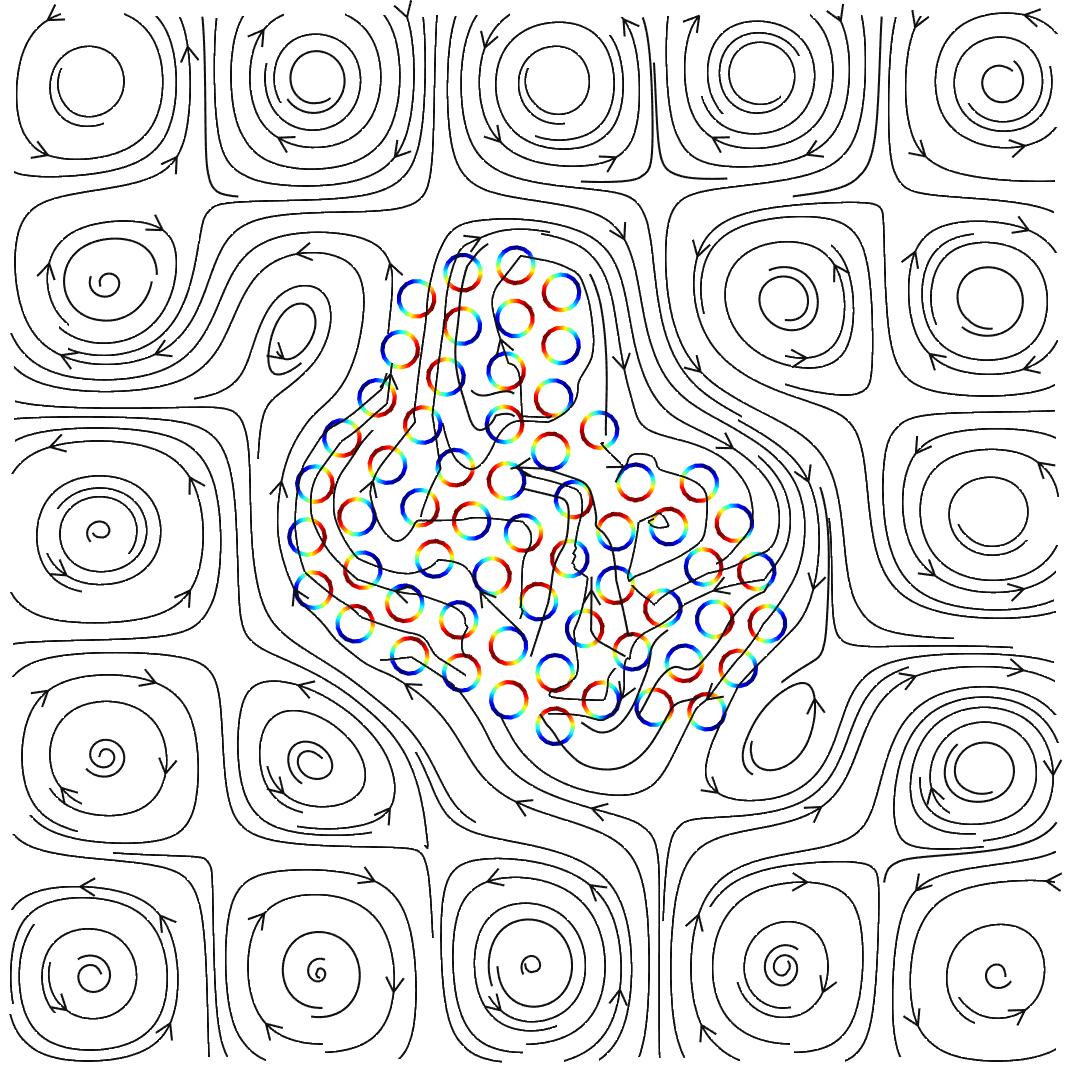
\includegraphics[width=0.4\textwidth]{TG_5000.png}
    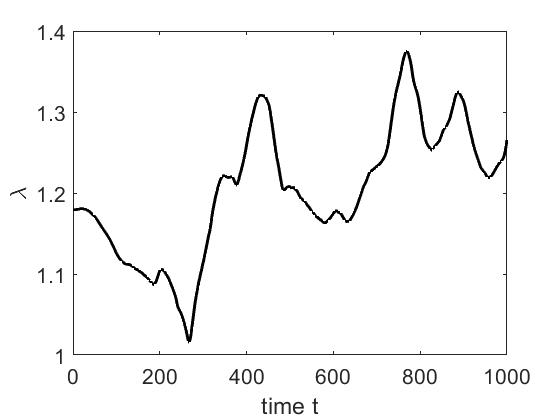
\includegraphics[width=0.4\textwidth]{TG_dist.jpg}
  \end{center}
  \vspace{-20pt}  
  \caption{\label{fig:TG_1} Snapshots of simulation using boundary condition \eqref{eq:bcs}(b) in a Taylor-Green flow when $V_0=0.1$ and $l=0.5$.}
\end{figure}


Similar to shear flow simulations, we then place equilibrium states of all boundary conditions \eqref{eq:bcs} in a rotating Taylor-Green Flow with a length scale $l$
\begin{equation}
\uu_\infty(\xx) = V_0 \left(-\cos(l{\bf e}_x\cdot\xx)\sin(l{\bf e}_y\cdot\xx){\bf e}_x+\sin(l{\bf e}_x\cdot\xx)\cos(l{\bf e}_y\cdot\xx){\bf e}_y\right).
\end{equation}
%
The magnitude of the vortex flow is controlled by the velocity scale $V_0$.


\subsection{Steady-State Structure Confined in Narrow Channels}



\begin{figure}
  \begin{center}
  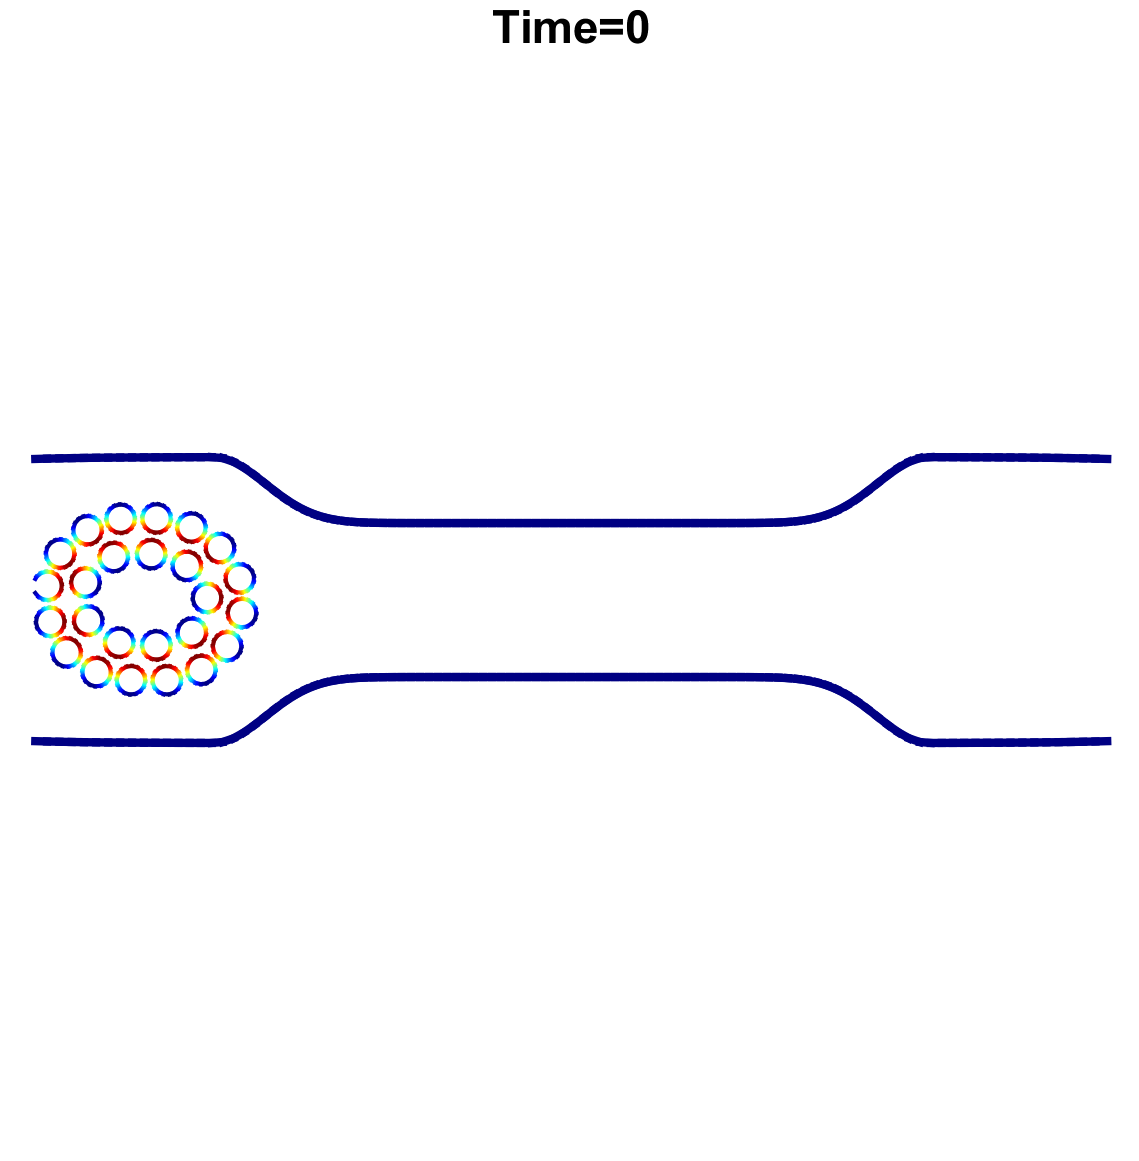
\includegraphics[width=0.4\textwidth]{VesConf_0.png}
  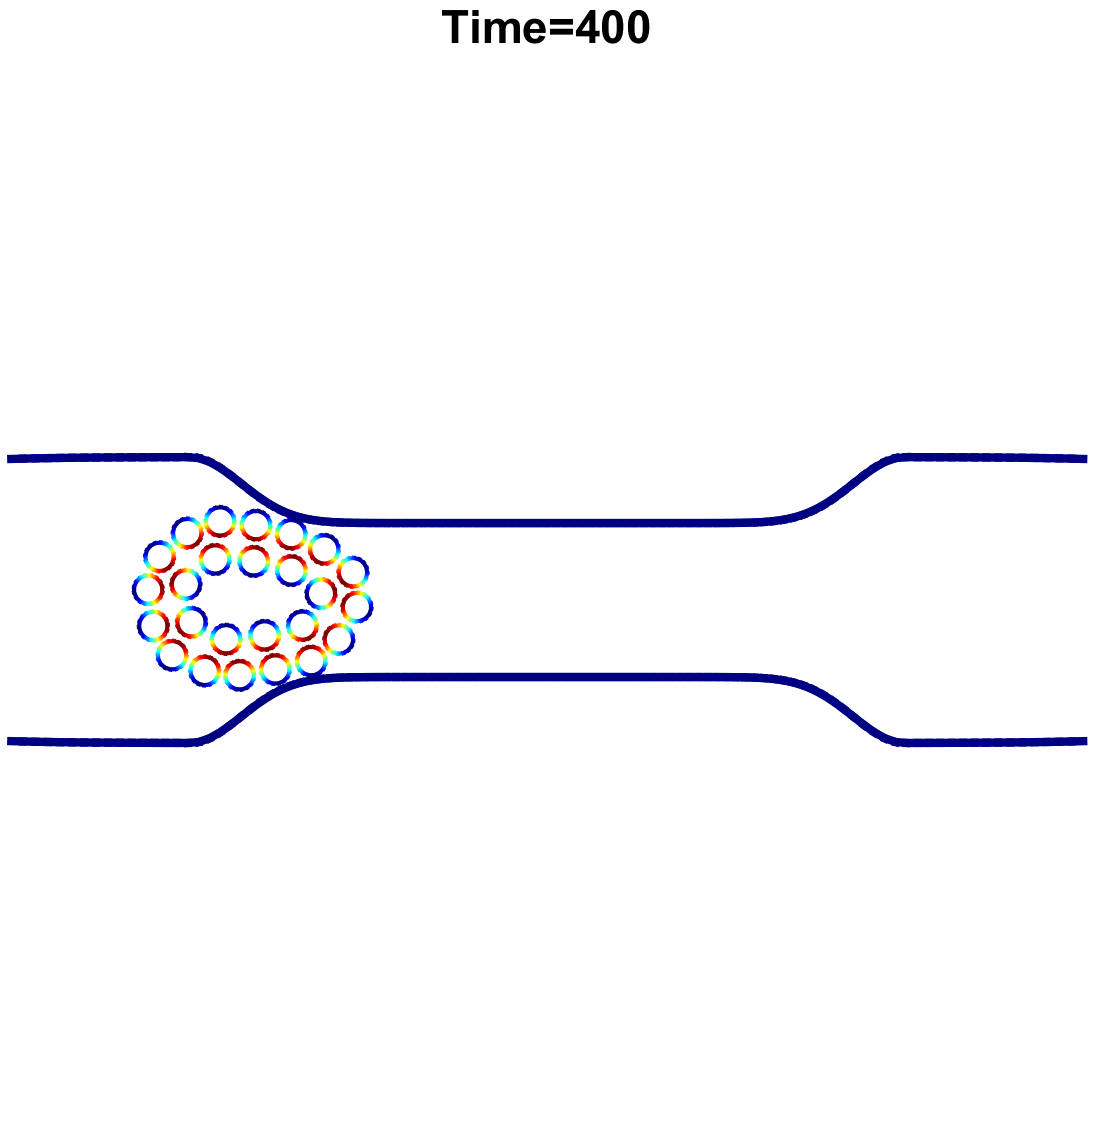
\includegraphics[width=0.4\textwidth]{VesConf_2000.png}\\
  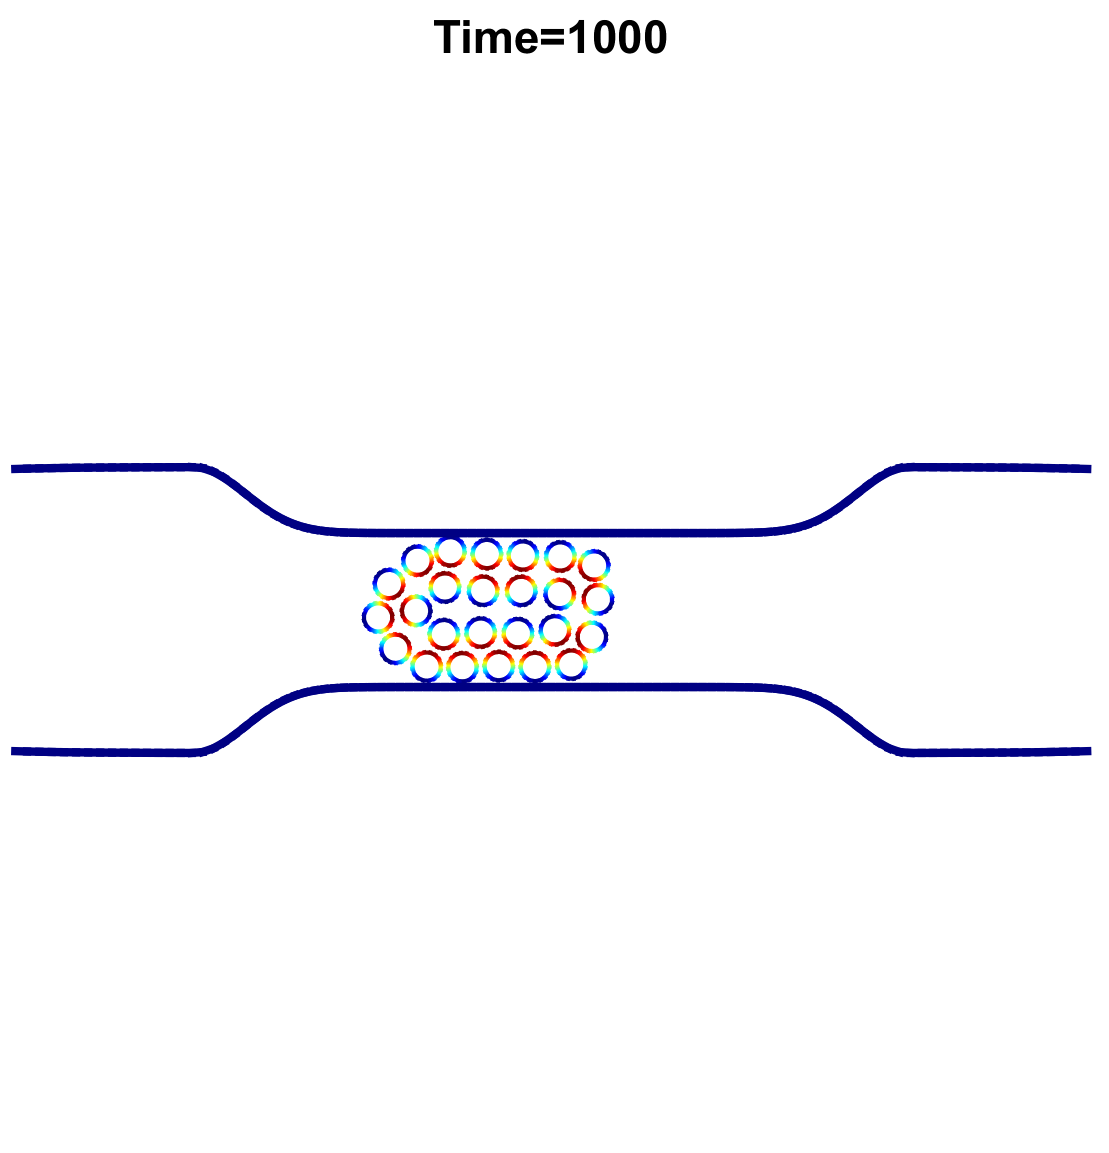
\includegraphics[width=0.4\textwidth]{VesConf_5000.png}
  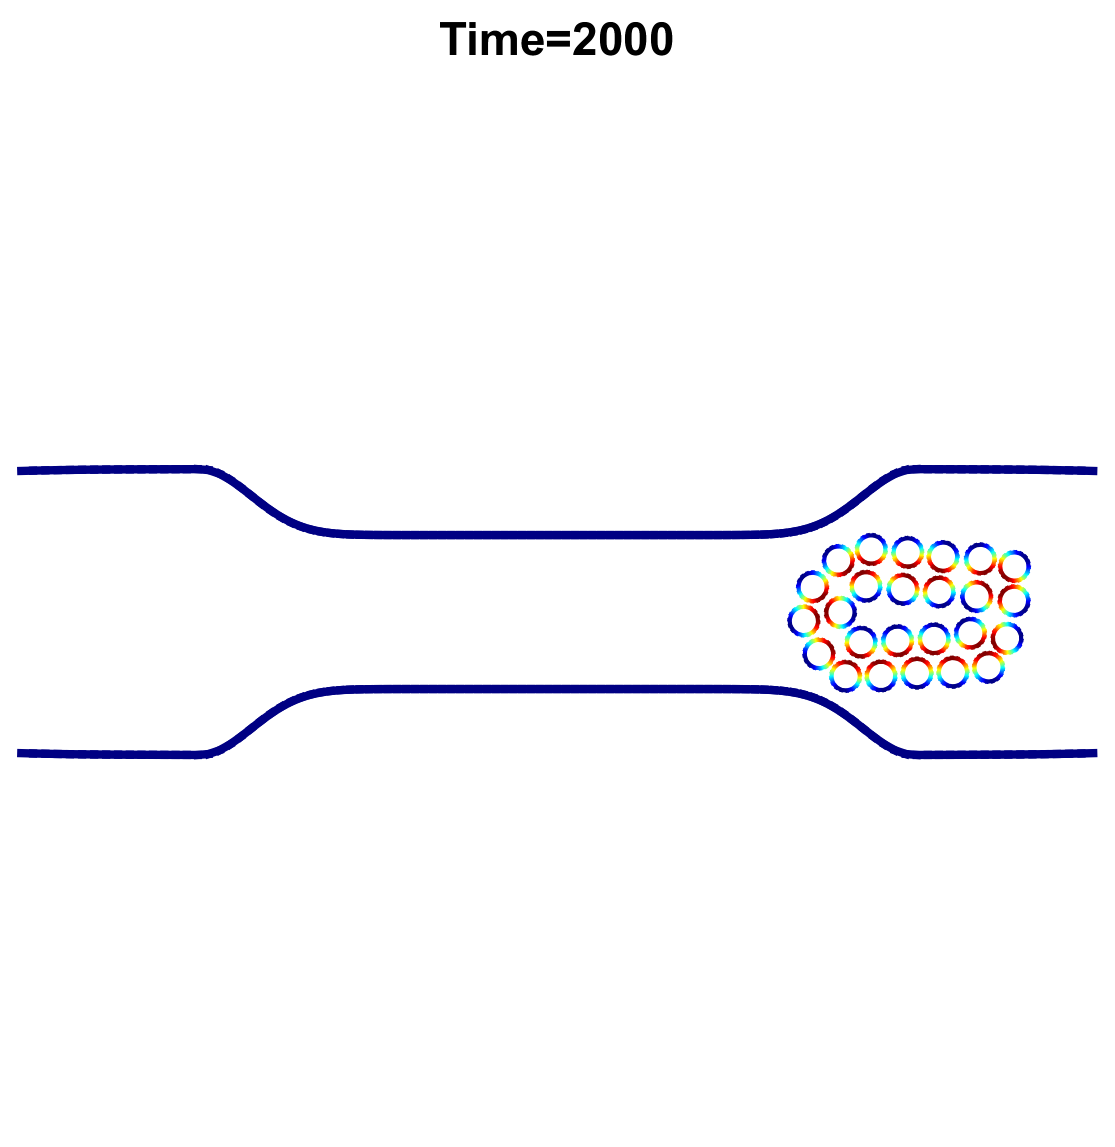
\includegraphics[width=0.4\textwidth]{VesConf_10000.png}
  \end{center}
  \vspace{-20pt}  
  \caption{\label{fig:confined_vesicle} A JP vesicle confined in a narrow channel where $N_b=25$ and $\dot\gamma=0.01$.  }
\end{figure}




\begin{figure}
  \begin{center}
  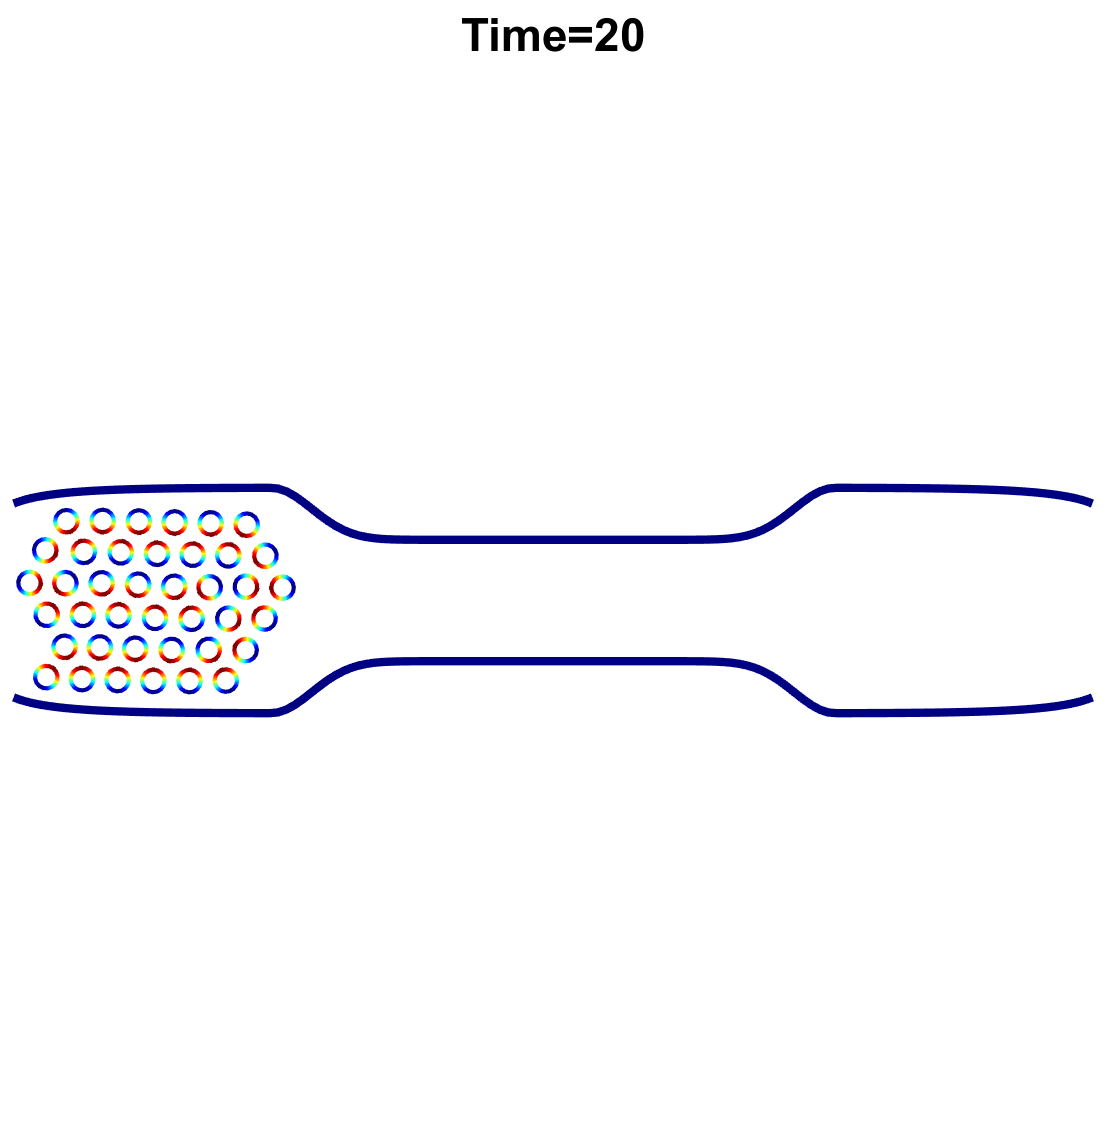
\includegraphics[width=0.4\textwidth]{MultConf_100.png}
  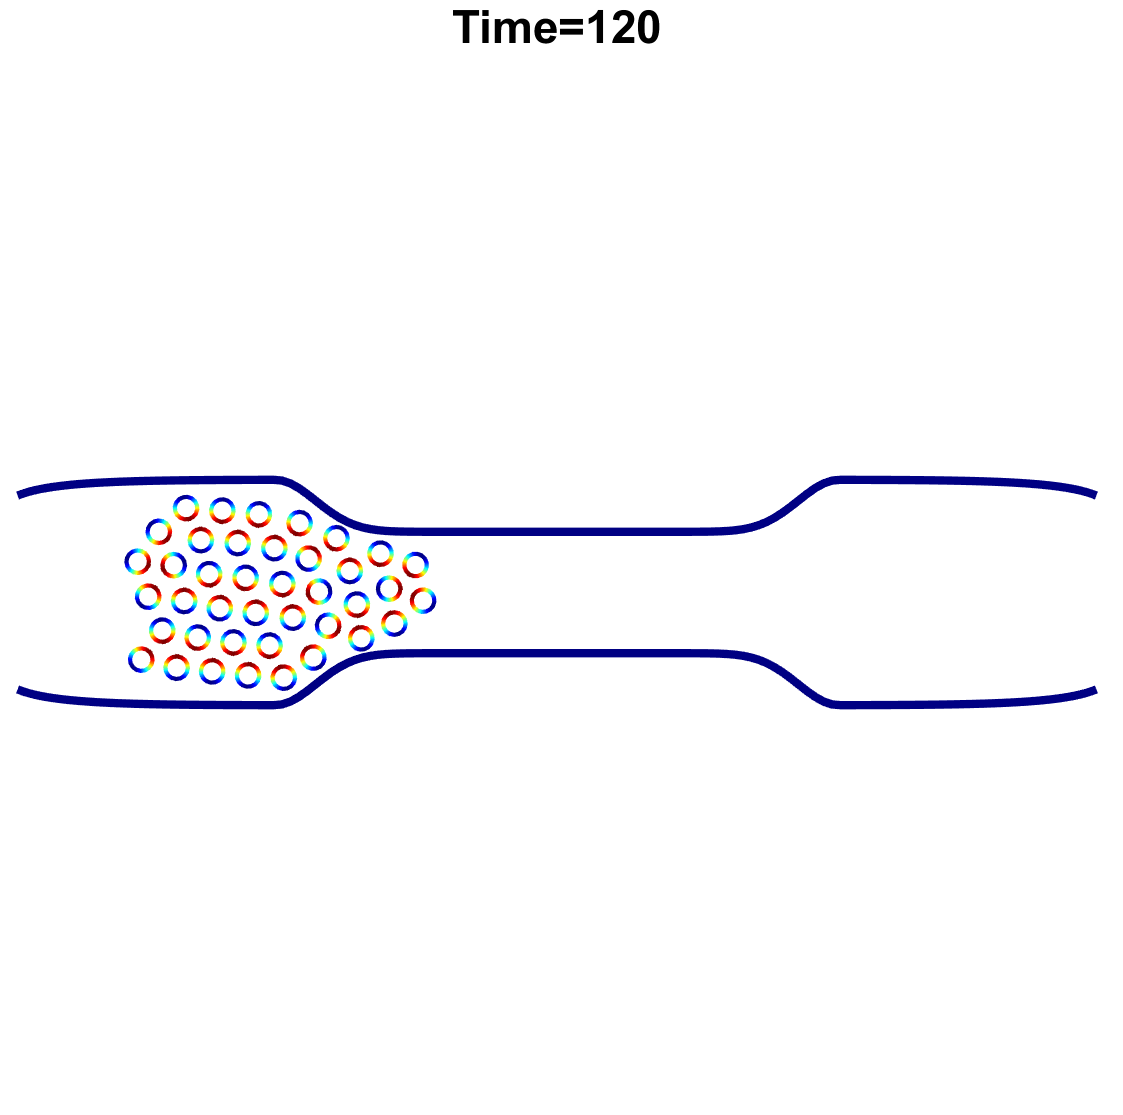
\includegraphics[width=0.4\textwidth]{MultConf_600.png}\\
  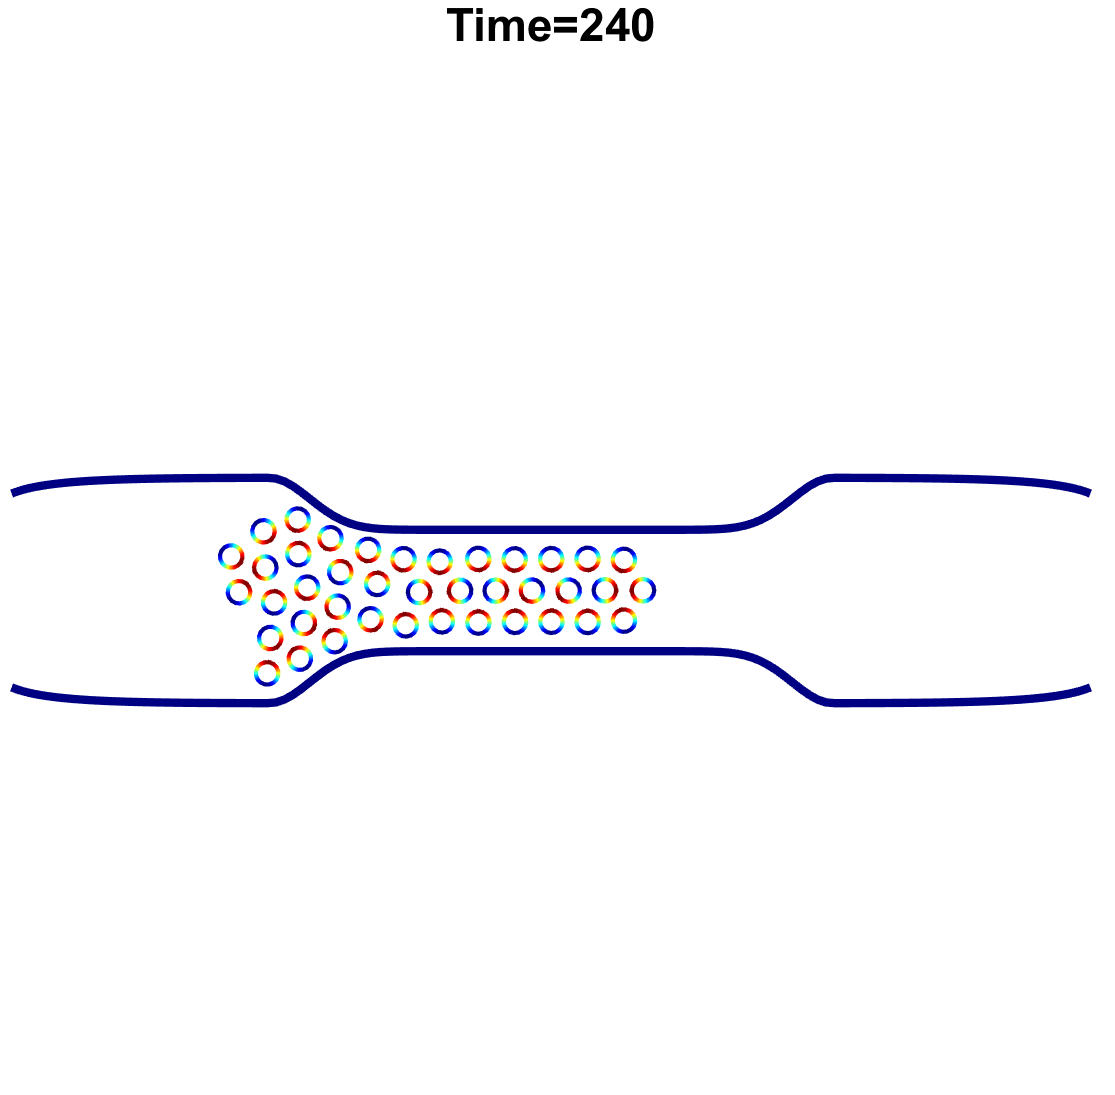
\includegraphics[width=0.4\textwidth]{MultConf_1200.png}
  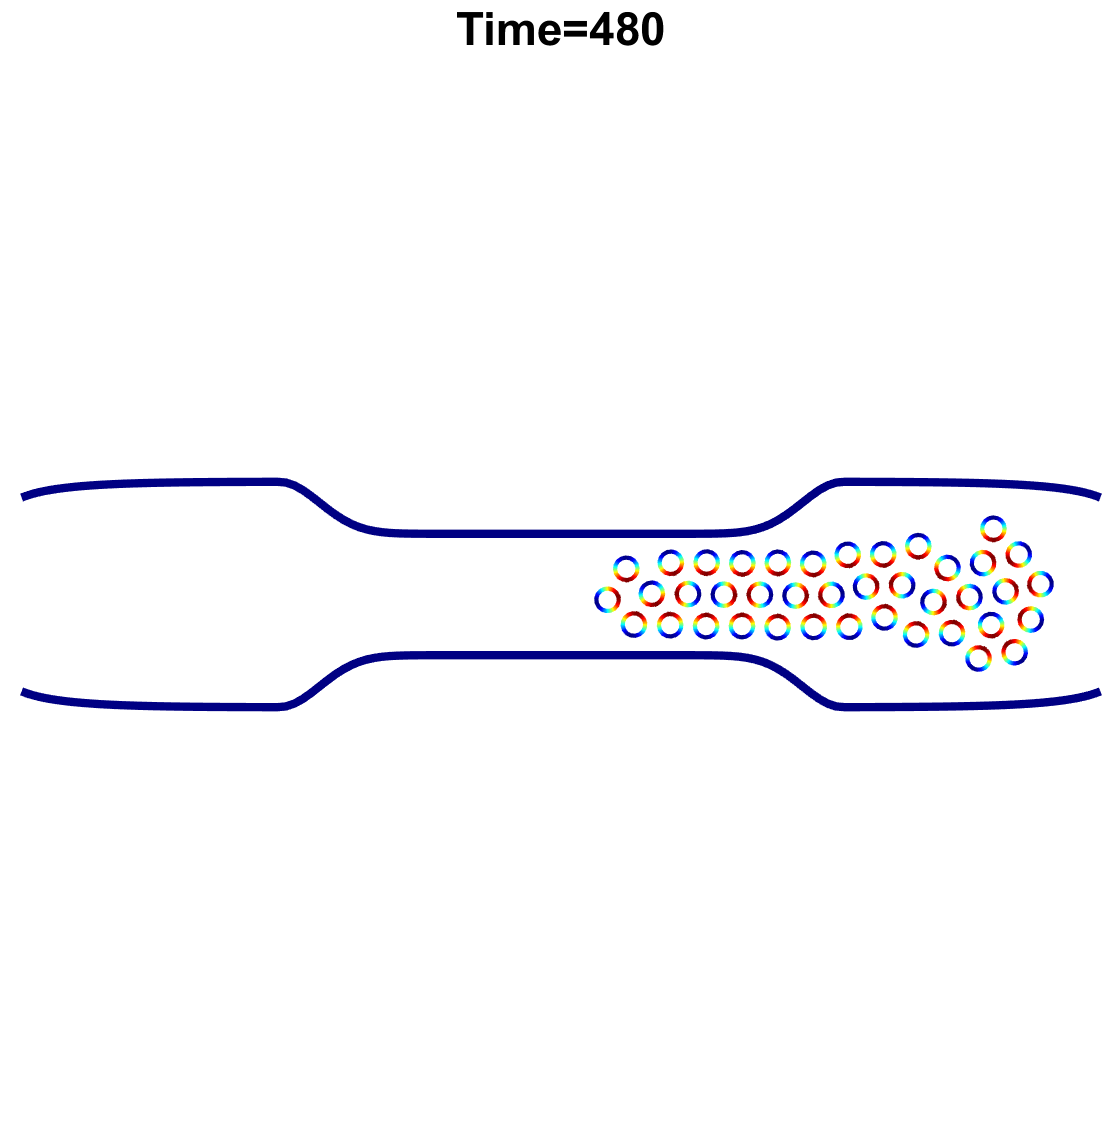
\includegraphics[width=0.4\textwidth]{MultConf_2400.png}
  \end{center}
  \vspace{-20pt}  
  \caption{\label{fig:confined_lamellar} A JP multi-lamellar structure confined in a narrow channel where $N_b=40$ and $\dot\gamma=0.05$.  }
\end{figure}


\section{Conclusions}




%%%

% If in two-column mode, this environment will change to single-column
% format so that long equations can be displayed. Use
% sparingly.
%\begin{widetext}
% put long equation here
%\end{widetext}

% figures should be put into the text as floats.
% Use the graphics or graphicx packages (distributed with LaTeX2e)
% and the \includegraphics macro defined in those packages.
% See the LaTeX Graphics Companion by Michel Goosens, Sebastian Rahtz,
% and Frank Mittelbach for instance.
%
% Here is an example of the general form of a figure:
% Fill in the caption in the braces of the \caption{} command. Put the label
% that you will use with \ref{} command in the braces of the \label{} command.
% Use the figure* environment if the figure should span across the
% entire page. There is no need to do explicit centering.

% \begin{figure}
% \includegraphics{}%
% \caption{\label{}}
% \end{figure}

% Surround figure environment with turnpage environment for landscape
% figure
% \begin{turnpage}
% \begin{figure}
% \includegraphics{}%
% \caption{\label{}}
% \end{figure}
% \end{turnpage}

% tables should appear as floats within the text
%
% Here is an example of the general form of a table:
% Fill in the caption in the braces of the \caption{} command. Put the label
% that you will use with \ref{} command in the braces of the \label{} command.
% Insert the column specifiers (l, r, c, d, etc.) in the empty braces of the
% \begin{tabular}{} command.
% The ruledtabular enviroment adds doubled rules to table and sets a
% reasonable default table settings.
% Use the table* environment to get a full-width table in two-column
% Add \usepackage{longtable} and the longtable (or longtable*}
% environment for nicely formatted long tables. Or use the the [H]
% placement option to break a long table (with less control than 
% in longtable).
% \begin{table}%[H] add [H] placement to break table across pages
% \caption{\label{}}
% \begin{ruledtabular}
% \begin{tabular}{}
% Lines of table here ending with \\
% \end{tabular}
% \end{ruledtabular}
% \end{table}

% Surround table environment with turnpage environment for landscape
% table
% \begin{turnpage}
% \begin{table}
% \caption{\label{}}
% \begin{ruledtabular}
% \begin{tabular}{}
% \end{tabular}
% \end{ruledtabular}
% \end{table}
% \end{turnpage}

% Specify following sections are appendices. Use \appendix* if there
% only one appendix.
%\appendix
%\section{}

% If you have acknowledgments, this puts in the proper section head.
\begin{acknowledgments}
We thank Dr. S\'ebastien Michelin and Dr. Cecile Cottin-Bizzonne from LadHyX - Ecole Polytechnique Institut Polytechnique de Paris for organizing the focus-session ``interfacial active matter'' in the conference APS-DFD 2021 and the invitation of submitting a special collection paper. 

% put your acknowledgments here.
\end{acknowledgments}

% Create the reference section using BibTeX:
\bibliography{reference}

\end{document}
%
% ****** End of file apstemplate.tex ******

